% % % % % % % % % % % % % % % % % % % % % % % % % % % % % % % % % % % % % % % % % % % %
%                                                                                     %
% Short Sectioned Assignment LaTeX Template Version 1.0 (5/5/12)                      %
% This template has been downloaded from: http://www.LaTeXTemplates.com               %
%                                                                                     %
% Original author:  Frits Wenneker (http://www.howtotex.com)                          %
%                                                                                     %
% Modified by: Fco Javier Sueza Rodríguez (fcosueza@disroot.org)                      %
%                                                                                     %
% Changes:                                                                            %
%	    - Custom Chapters, Sections and Subsections (titlesec package)                %
%           - Document type scrbook (oneside)                                         %
%           - Use babel-lang-spanish package and marvosym                             %
%           - Use hyperref, enumitem, tcolorbox and glossaries packages               %
%           - Use Time New Roman (mathptmx), Helvetic and Courier fonts               %
%                                                                                     %
% License: CC BY-NC-SA 3.0 (http://creativecommons.org/licenses/by-nc-sa/3.0/)        %
%                                                                                     %
% % % % % % % % % % % % % % % % % % % % % % % % % % % % % % % % % % % % % % % % % % % %

%-----------------------------------------------%
%	              Packages                  %
%-----------------------------------------------%

\documentclass[paper=a4, fontsize=11pt, oneside]{scrbook}

% ---- Text Input/Output ----- %

\usepackage[T1]{fontenc}
\usepackage[utf8]{inputenc}
\usepackage{mathptmx}
\usepackage[scaled=.92]{helvet}
\usepackage{courier}
\usepackage[indent=12pt]{parskip}

\usepackage{geometry}
\geometry{verbose,tmargin=3cm,bmargin=3cm,lmargin=2.6cm,rmargin=2.6cm}

% ---- Language ----- %

\usepackage[spanish]{babel}
\usepackage{marvosym}

% ---- Another packages ---- %

\usepackage{amsmath,amsfonts,amsthm}
\usepackage{graphics,graphicx}
\usepackage{titlesec}
\usepackage{fancyhdr}
\usepackage{tcolorbox}
\usepackage{hyperref}
\usepackage{enumitem}
\usepackage[automake]{glossaries}

%--------------------------------------------------------------------%
%                      Customizing Document                          %
%--------------------------------------------------------------------%


% ----------- Custom Chapters, Sections and Subsections -------------- %

\titleformat{\chapter}[display]
			{\bfseries\Huge}
			{Tema \ \thechapter} {0.5ex}
			{\vspace{1ex}\centering}

\titleformat{\section}[hang]
			{\bfseries\Large}
			{\thesection}{0.5em}{}

\titleformat{\subsection}[hang]
			{\bfseries\large}
			{\thesubsection}{0.5em}{}

\titleformat{\subsubsection}[hang]
			{\bfseries\large}
			{\thesubsubsection}{0.5em}{}

\hypersetup{
    colorlinks=true,
    linkcolor=black,
    urlcolor=magenta
}

% ------------------- Custom heaaders and footers ------------------- %

\pagestyle{fancyplain}

\fancyhead[]{}
\fancyfoot[L]{}
\fancyfoot[C]{}
\fancyfoot[R]{\thepage}

\renewcommand{\headrulewidth}{0pt} % Remove header underlines
\renewcommand{\footrulewidth}{0pt} % Remove footer underlines

\setlength{\headheight}{13.6pt} % Customize the height of the header

% --------- Numbering equations, figures and tables ----------------- %

\numberwithin{equation}{section} % Number equations within sections
\numberwithin{figure}{section} % Number figures within sections
\numberwithin{table}{section} % Number tables within sections

% ------------------------ New Commands ----------------------------- %

\newcommand{\horrule}[1]{\rule{\linewidth}{#1}} % Create horizontal rule command


%----------------------------------------------------------------------------------------
%	TÍTULO Y DATOS DEL ALUMNO
%----------------------------------------------------------------------------------------

\title{
\vspace{10ex}
\normalfont \normalsize
\Huge \textbf{Tarea 5: Manipulación de Datos de una Base de Datos Relacional Utilizando MySQL}
}
\author{Francisco Javier Sueza Rodríguez}
\date{\normalsize\today}

%----------------------------------------------------------------------------------------
%                                     DOCUMENTO
%----------------------------------------------------------------------------------------
\begin{document}

\maketitle

\thispagestyle{empty}

\vspace{62ex}

\begin{center}
    \begin{tabular}{l l}
        \textbf{Centro}: & IES Aguadulce \\
        \textbf{Ciclo Formativo}: & Desarrollo Aplicaciones Web (Distancia)\\
        \textbf{Asignatura}: & Bases de Datos\\
        \textbf{Tema}: & Tema 5 - Tratamiento de Datos\\
    \end{tabular}
\end{center}

\newpage

\tableofcontents

\newpage

\listoffigures

\newpage

\section{Caso Práctico}

Ana sigue trabajando con la BD anterior de la empresa CUIDA TU CUERPO. Ahora deben trabajar con la información y deben utilizar las sentencias INSERT, DELETE y UPDATE del lenguaje SQL. También utilizarán la herramienta gráfica de MySQL para realizar algunas de estas operaciones.

De la misma forma que en la unidad anterior, tendrás que apoyar a Ana para realizar las sentencias y operaciones necesarias que se piden sobre la misma BD

\section{Enunciado}
Para poder acceder a información de una Base de Datos, ésta debe estar creada y debe contener registros previamente. Por tanto, lo primero que debes realizar es descargar el script que contiene las tablas y datos que encontrarás en el apartado 2.- ``Información de interés'', además de seguir todos los consejos y recomendaciones para elaborar esta tarea que en dicho apartado se explican.

Lo que realmente se pide en la tarea es que ayudes a Ana redactando las sentencias SQL que ejecuten cada una de las siguientes consultas correctamente en MySQL.

Debes realizar cada una de las siguientes operaciones utilizando para ello las indicaciones de cada apartado:

\subsection{Apartado A}
Utilizando la \textbf{interfaz gráfica} de \textbf{MySQL Workbench} (sin utilizar sentencias SQL), debes realizar las siguientes operaciones adjuntando al menos \textbf{DOS capturas} de pantalla de cada subapartado. En las capturas de pantalla es totalmente obligatorio disponer las ventanas de forma que se visualice tu usuario de la plataforma (foto y nombre).

\begin{enumerate}
    \item  Insertar un nuevo registro en la tabla CLIENTE con los siguientes datos:

    \begin{itemize}
        \item DNI: 88256456M
        \item Nombre: Jacinto
        \item Apellidos: Martín Lago
        \item Teléfono: 658986241
        \item Descuento: 10
        \item Baja: No
    \end{itemize}

    \item A la única cita que tenemos el día 18-12-2022 le vamos a modificar la duración por 55 minutos, la hora a las 12:00 y el precio a 25.99. Modifica los datos en la tabla correspondiente.

    \item Por políticas de la empresa, se ha decidido eliminar los Anabolizantes de nuestros productos. Hay que borrar el registro de la tabla correspondiente.
\end{enumerate}

\subsection{Apartado B}
Utilizando \textbf{sentencias SQL} en la herramienta \textbf{MySQL Workbench}, debes realizar las siguientes operaciones indicando la sentencia que ejecutarías para realizar cada uno de los subapartados:

\begin{enumerate}
    \item Insertar los siguientes datos en la tabla CITA teniendo en cuenta que debes insertar sólo los valores necesarios en los campos correspondientes.

    \begin{figure}[H]
        \centering
        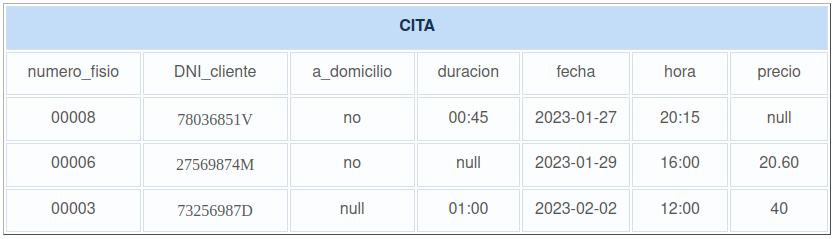
\includegraphics[scale=0.50]{tabla-enunciado.png}
        \caption{Datos para introducir en la tabla CITA}
    \end{figure}

    \item Incrementar un 15\% el precio de todos los productos que sean vendajes (da igual el tipo de vendaje). (Debes hacerlo con una única sentencia).

    \item Eliminar las citas cuyo precio sea menor de 25 y estén asignadas a fisioterapeutas que no estén trabajando actualmente. (Debes hacerlo con una única sentencia).

    \item Incrementa en 5 unidades el descuento de los clientes que han tenido 3 o más citas en 2022, siempre y cuando no tengan ya un descuento superior a 60. (Debes hacerlo con una única sentencia)

    \item Insertar todos los profesionales que estén en estado ‘Despedido’ en la tabla PROFESIONALES\_BAJA, incluyendo además de los campos propios de la tabla PROFESIONALES, la duración de su jornada laboral. (Debes hacerlo con una única sentencia).

    \item Decrementar un año de experiencia a los profesores de pilates que han impartido menos de 3 clases en el último año. (Debes hacerlo con una única sentencia).

    \item Insertar en la tabla RANKING\_PRODUCTOS por cada producto, su código, su nombre y la cantidad total pedida, siempre y cuando se hayan vendido más de 15 unidades del producto. (Debes hacerlo con una única sentencia).

    \item Bloquear la tabla profesionales en modo lectura y la tabla cliente en modo escritura, seguidamente intenta actualizar el nombre del profesional con dni 56948768S por Jose. Luego, actualiza el nombre del cliente con dni 27256987J por Antonia. Muestra capturas del resultado de las distintas sentencias, explicando los resultados obtenidos.

    \item Inicia una transacción. Elimina todos los profesionales que su estado sea ‘despedido’. Deshacer la transacción y comprobar que los registros no han sido eliminados.
\end{enumerate}

\section{Solución}
En esta sección se incluyen las soluciones a los ejercicios propuestos en el enunciado anterior.

\subsection{Solución: Apartado A}
En primer lugar, vamos a usar la \textbf{interfaz gráfica} de \textbf{MySQL Workbench} para realizar la manipulación de las tablas de la base de datos creada.

\begin{enumerate}
    \item Primero hemos introducido un nuevo registro en la tabla \textbf{CLIENTE}. Desplegando el menú del schema creado, llamado \textbf{tarea5\_bd2223}, hemos pulsado en el \textbf{icono de la tabla} que nos aparece a la izquierda. Una vez ahí, hemos pulsado en el icono \textbf{Insert New Row} y rellenado los campos, pulsando posteriormente en el botón \textbf{Apply} abajo a la derecha. Como podemos ver en la siguiente captura.

    \begin{figure}[H]
        \centering
        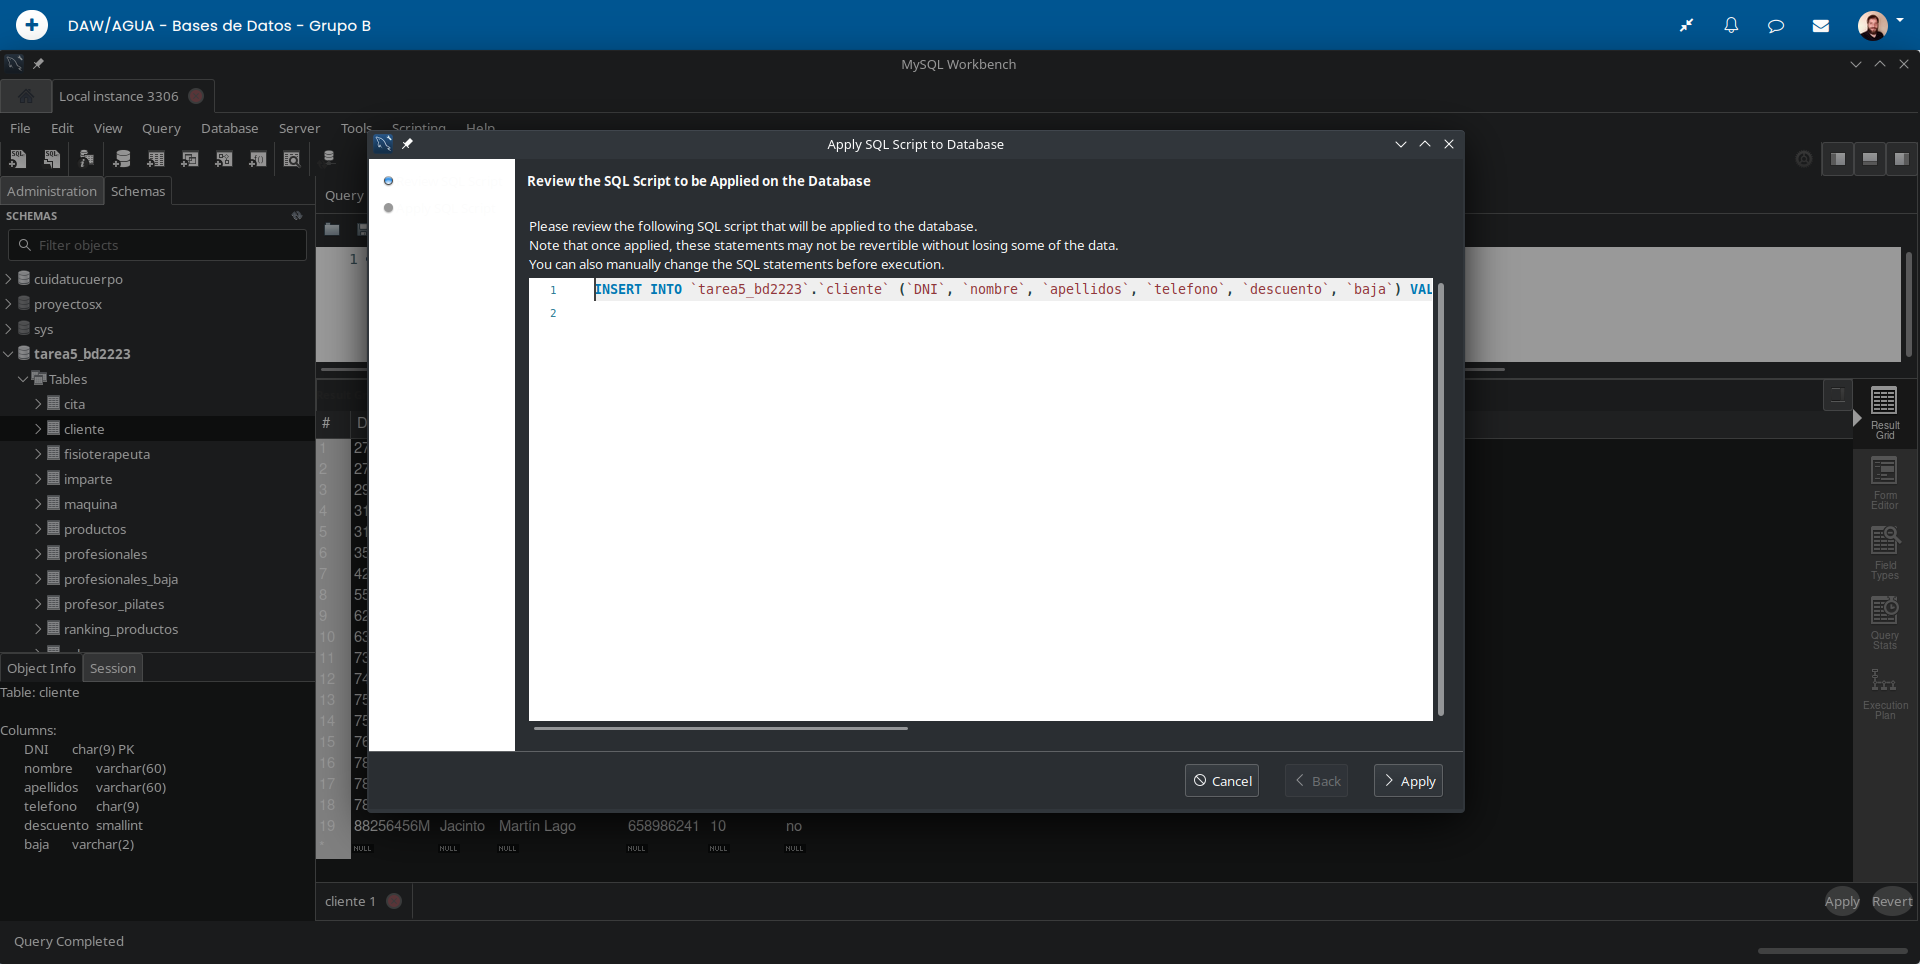
\includegraphics[scale=0.25]{workbench-1.png}
        \caption{Menu Apply de Workbench para añadir un registro}
    \end{figure}

    Una vez aplicado, la base de datos se ha actualizado y el registro a sido creado correctamente, lo que podemos comprobar cerrando la base de datos y haciendo una query \textbf{SELECT * FROM cliente;}, como vemos a continuación.

    \begin{figure}[H]
        \centering
        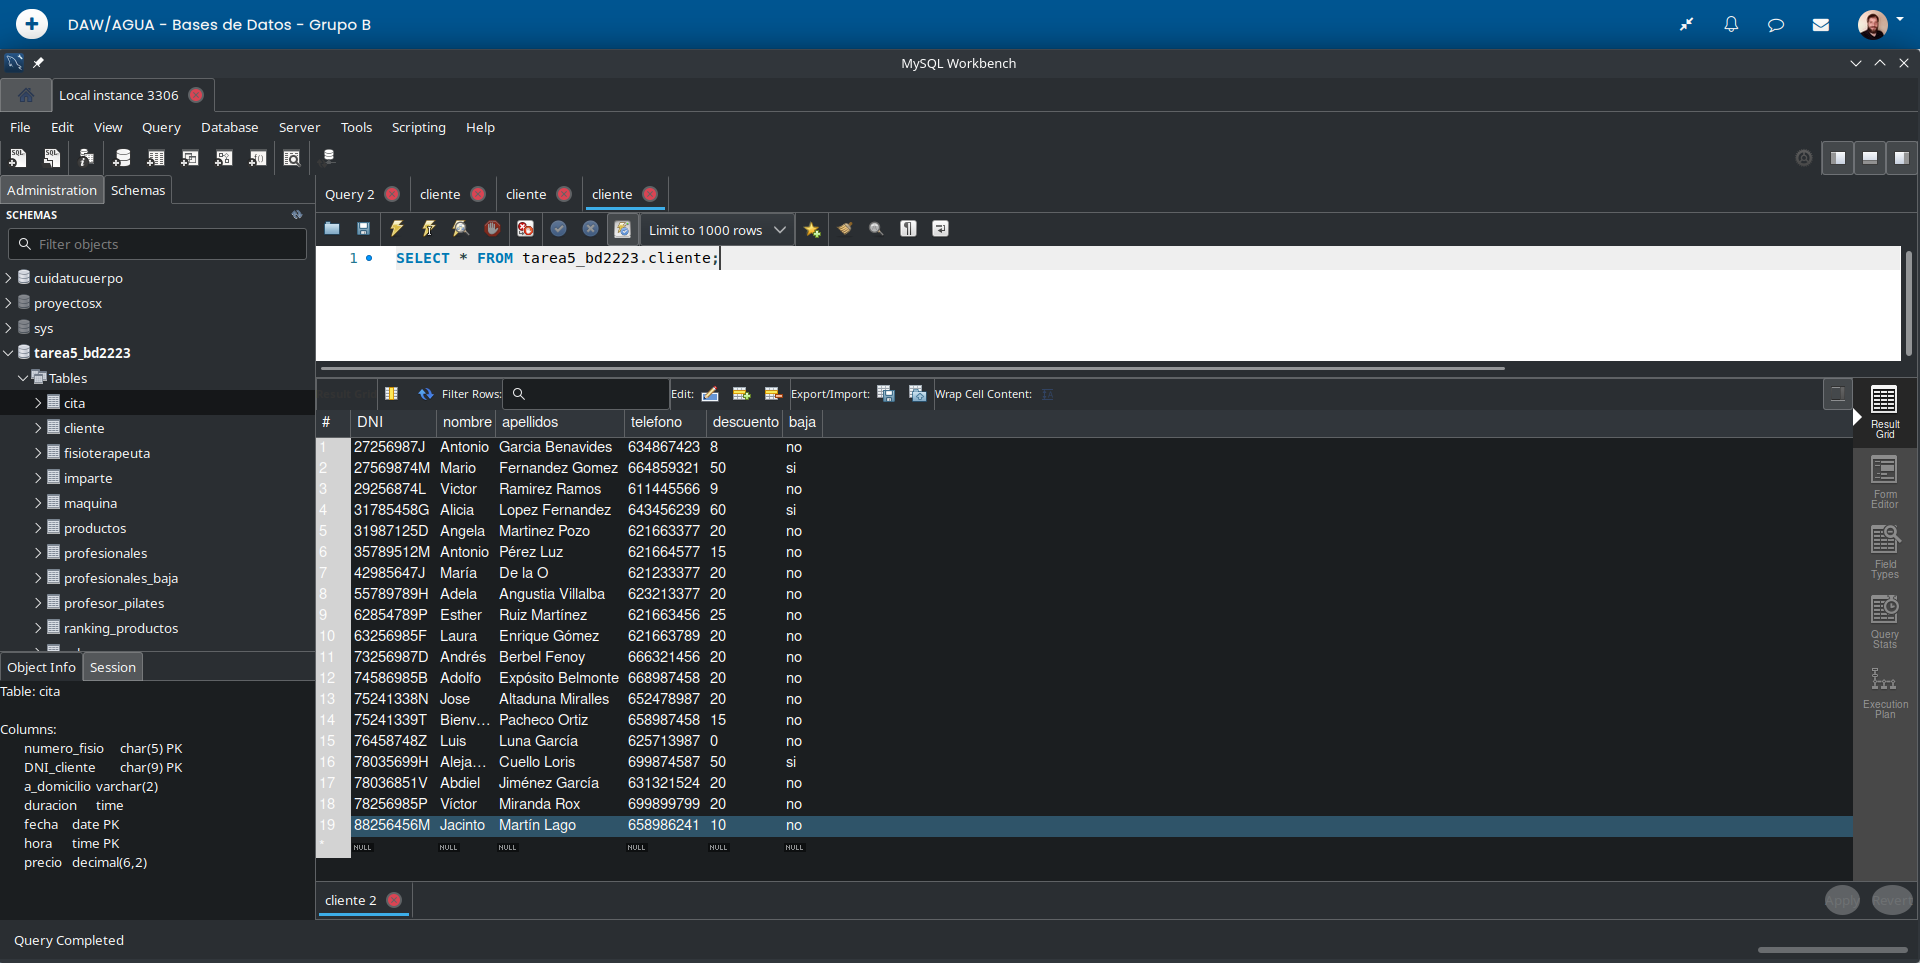
\includegraphics[scale=0.25]{workbench-2.png}
        \caption{Tabla cliente actualizada con el nuevo registro}
    \end{figure}

    \item En este punto hemos cambiado los valores de algunos campos en un registro. Para ello, hemos realizado el mismo procedimiento que en el punto anterior, pero en vez de pulsar en el icono para añadir una nueva fila, hemos pulsados en los campos del registro que queremos modificar y hemos cambiado sus valores, pulsando en Apply a continuación.

      \begin{figure}[H]
        \centering
        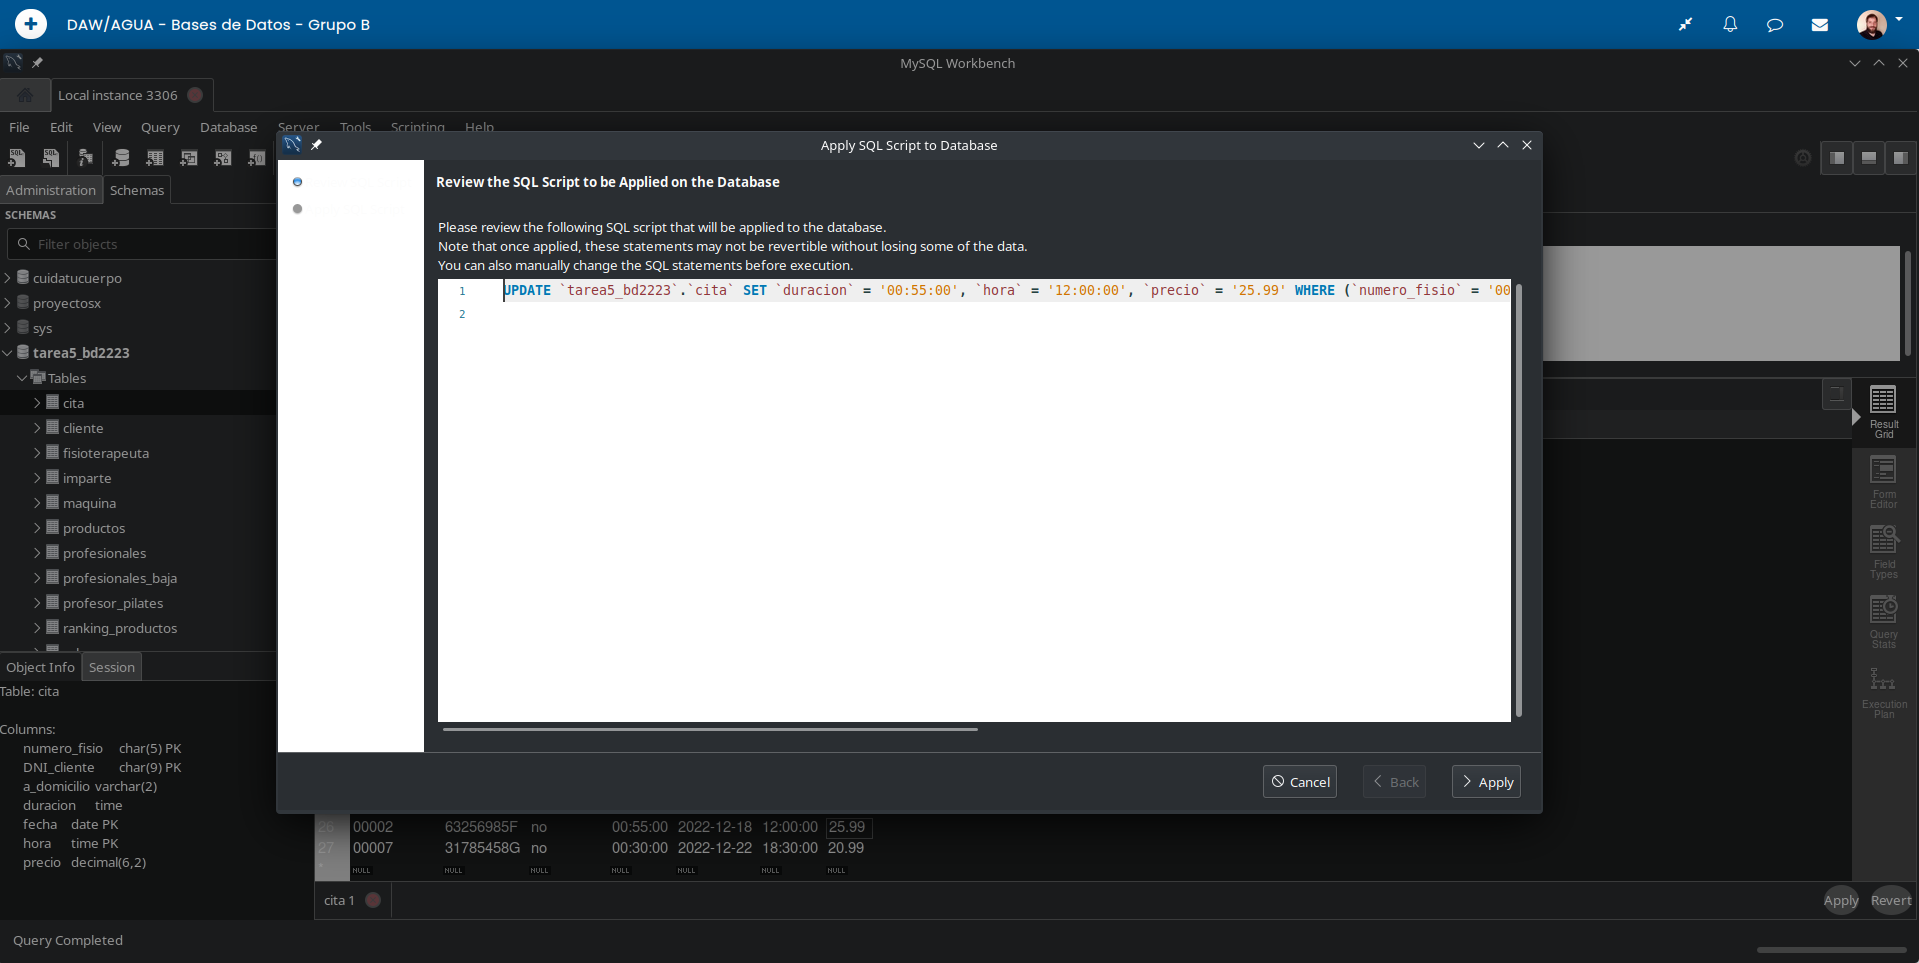
\includegraphics[scale=0.25]{workbench-3.png}
        \caption{Menu Apply de Workbench para modificar un registro}
    \end{figure}

    Para comprobar que el cambio se ha realizado correctamente, hemos realizado la consulta \textbf{SELECT * FROM cita WHERE fecha = "2022-12-18";}, comprobando en el resultado que el registro está modificado correctamente.

        \begin{figure}[H]
        \centering
        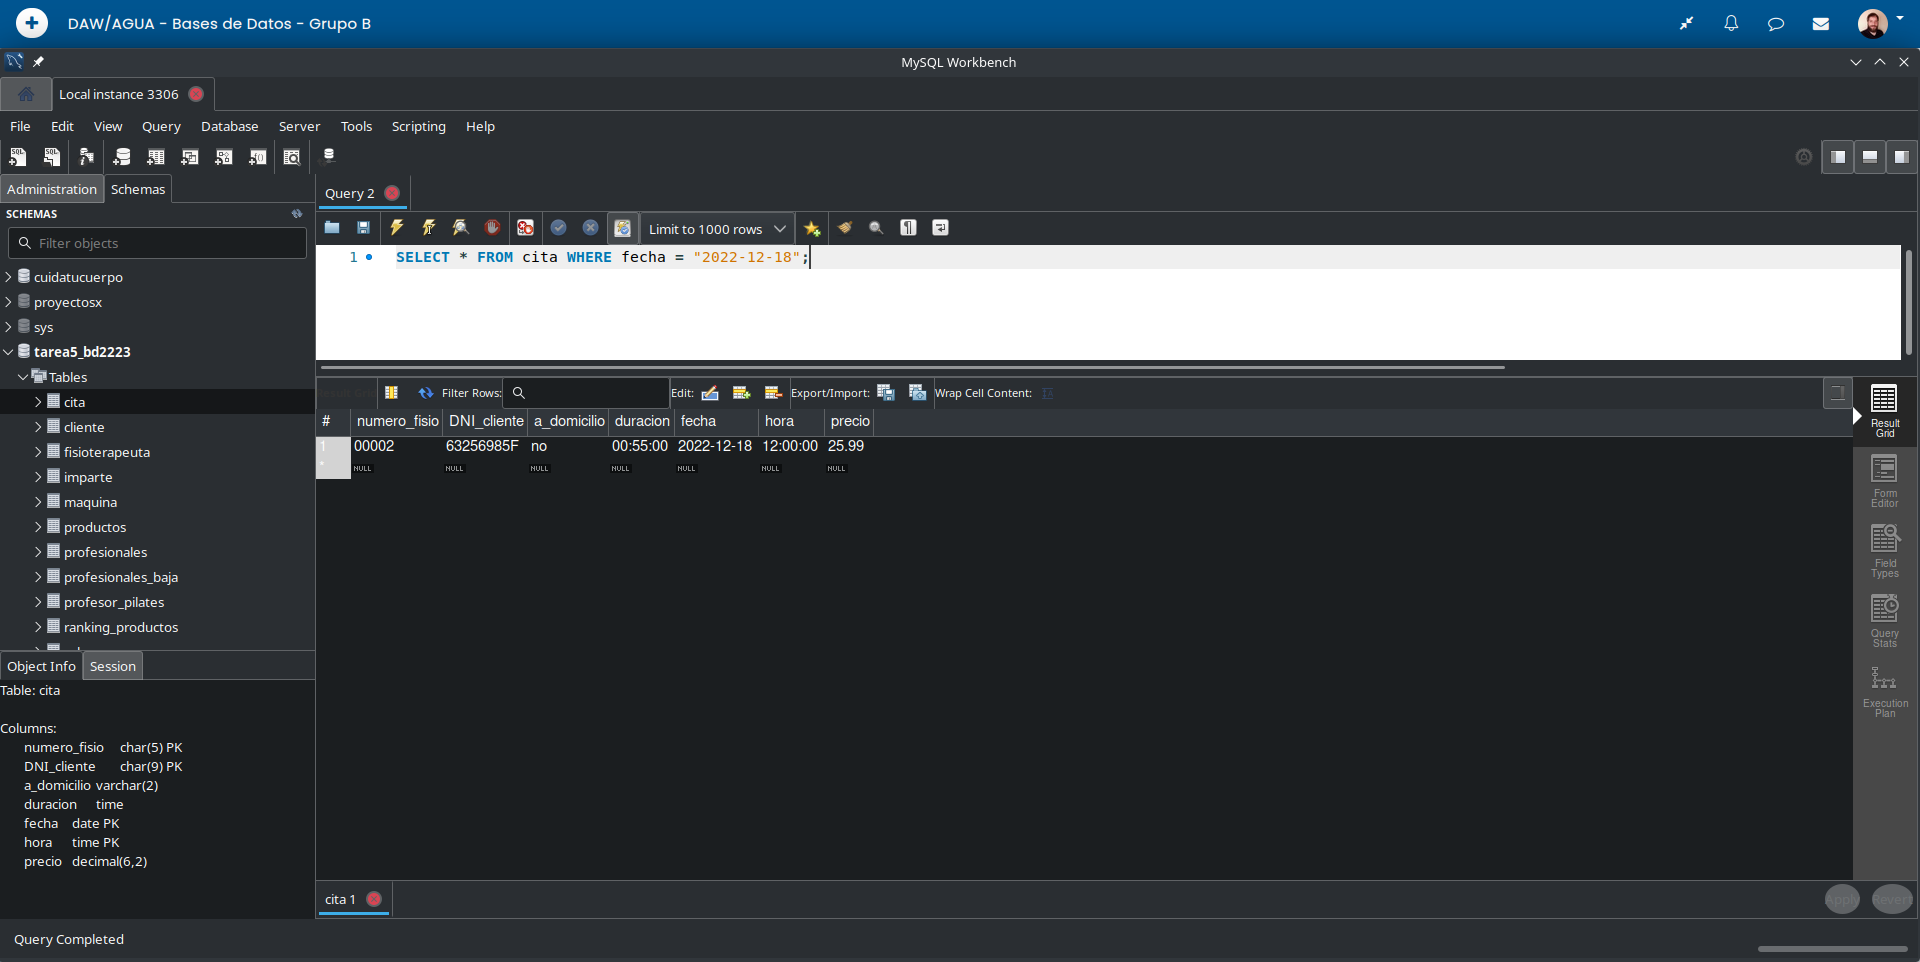
\includegraphics[scale=0.25]{workbench-4.png}
        \caption{Registro de la tabla cita modificado correctamente}
    \end{figure}

    \item Por último en este apartado, vamos a eliminar una registro de la tabla \textbf{productos}. En este caso, accediendo a la tabla como en los puntos anteriores, hemos seleccionado la fila que queremos borrar y pulsando con el botón derecho sobre ella, hemos elegido la opción \textbf{Delete Row(s)}. Tras lo que hemos pulsado en el botón Apply.

    \begin{figure}[H]
        \centering
        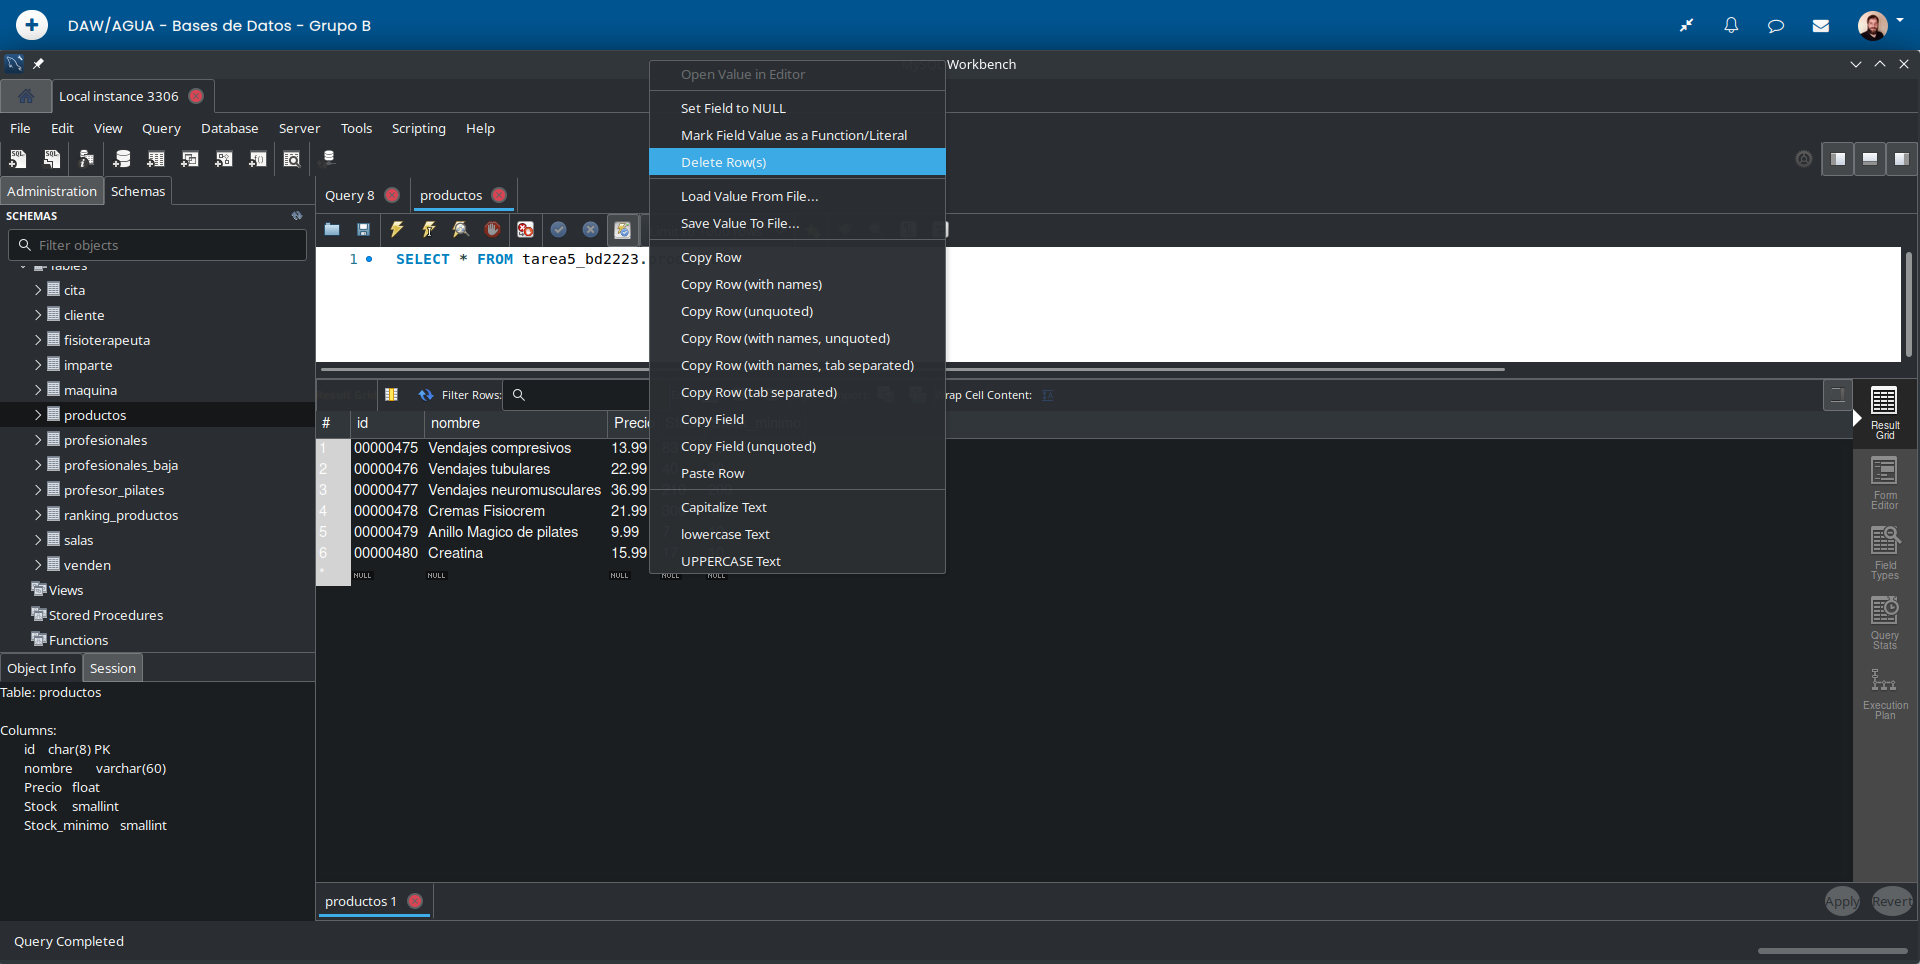
\includegraphics[scale=0.25]{workbench-5.png}
        \caption{Menu contextual del registro con la opción Delete Row(s)}
    \end{figure}

    Hemos realizado la consulta \textbf{SELECT * FROM productos;}, y como podemos ver en la siguiente captura, el registro de \textbf{Anabolizantes} se ha eliminado correctamente.

    \begin{figure}[H]
        \centering
        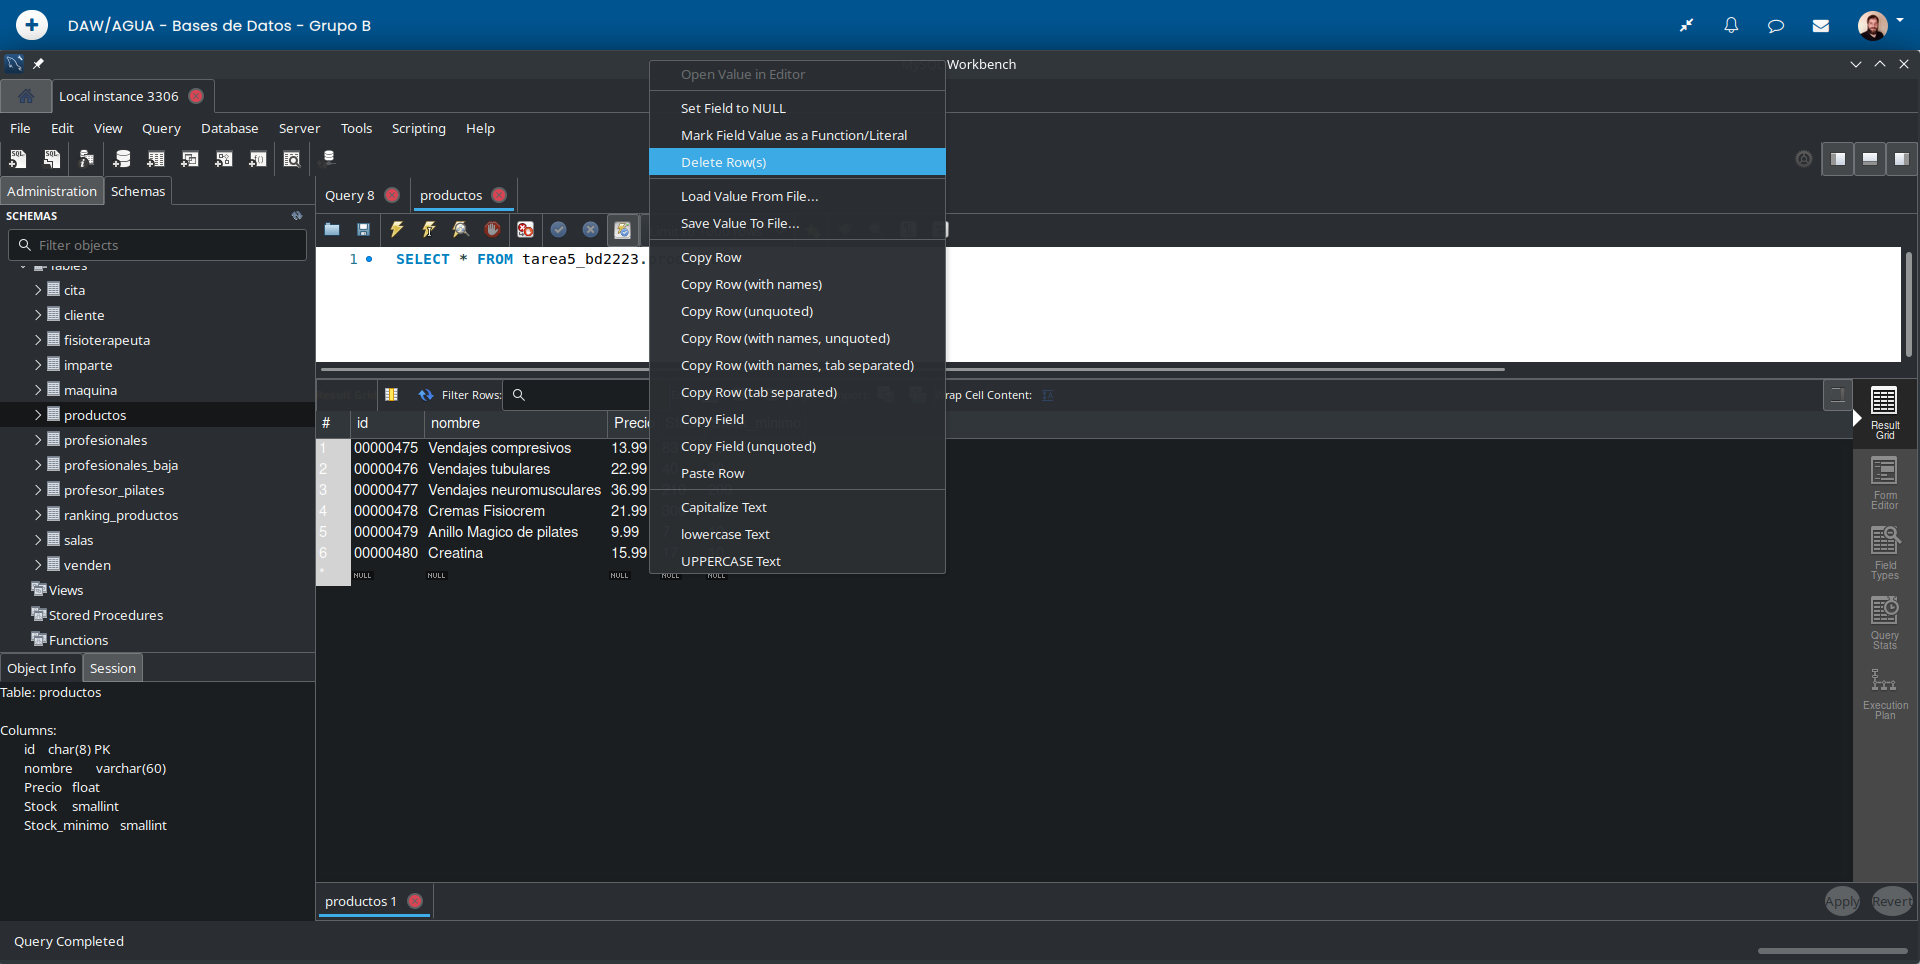
\includegraphics[scale=0.25]{workbench-5.png}
        \caption{Registro de anabolizantes borrado correctamente}
    \end{figure}
\end{enumerate}

\subsection{Apartado B}

En este apartado, vamos a realizar las modificaciones en la base de datos empleando \textbf{sentencias SQL}, en vez de mediante la interfaz gráfica.

\begin{enumerate}
    \item En primer lugar hemos añadido varias fila a la tabla citas. Podríamos haberlo realizado todo en una sentencia, si introdujéramos todos los datos de la columnas, pero como vamos a omitir los que tienen valor null, ya que el enunciado especifica que solo te introduzcan los campos necesarios, vamos a realizarlo en varias sentencias, acompañada cada una con una captura que muestra que se ha ejecutado correctamente.

    \begin{itemize}
        \item \textbf{Primera sentencia}:

        \begin{figure}[H]
            \begin{tcolorbox}[sharp corners, colback=yellow!30, colframe=white!20]
                \scriptsize
                \begin{verbatim}


INSERT INTO cita (numero_fisio, DNI_cliente, a_domicilio, duracion, fecha, hora)
VALUES ("00008", "78036851V", "no", "00:45", "2023-01-27", "20:15");
                \end{verbatim}
            \end{tcolorbox}
        \end{figure}

        \begin{figure}[H]
            \centering
            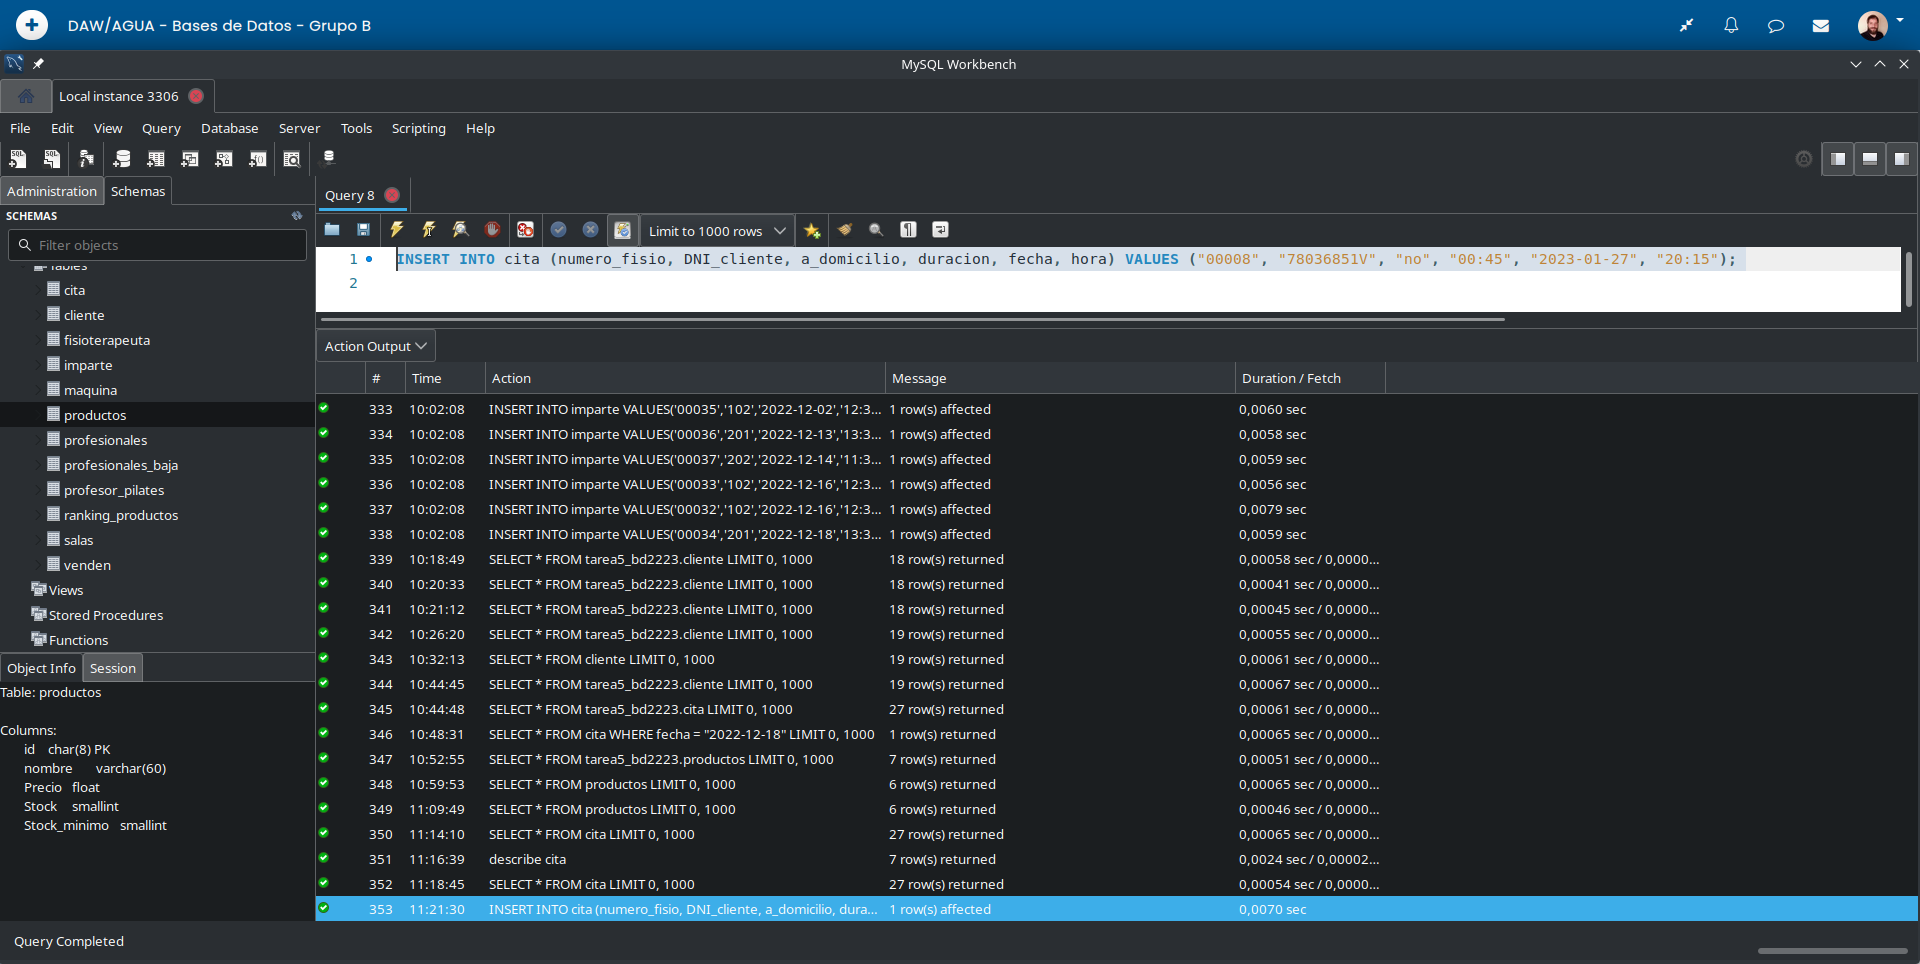
\includegraphics[scale=0.23]{sql-1.1.png}
            \caption{Ejecución de la primera sentencia}
        \end{figure}

        \item \textbf{Segunda sentencia}:

        \begin{figure}[H]
            \begin{tcolorbox}[sharp corners, colback=yellow!30, colframe=white!20]
                \scriptsize
                \begin{verbatim}


INSERT INTO cita (numero_fisio, DNI_cliente, a_domicilio, fecha, hora, precio)
VALUES ("00006", "27569874M", "no", "2023-01-29", "16:00", "20.60");
                \end{verbatim}
            \end{tcolorbox}
        \end{figure}

        \begin{figure}[H]
            \centering
            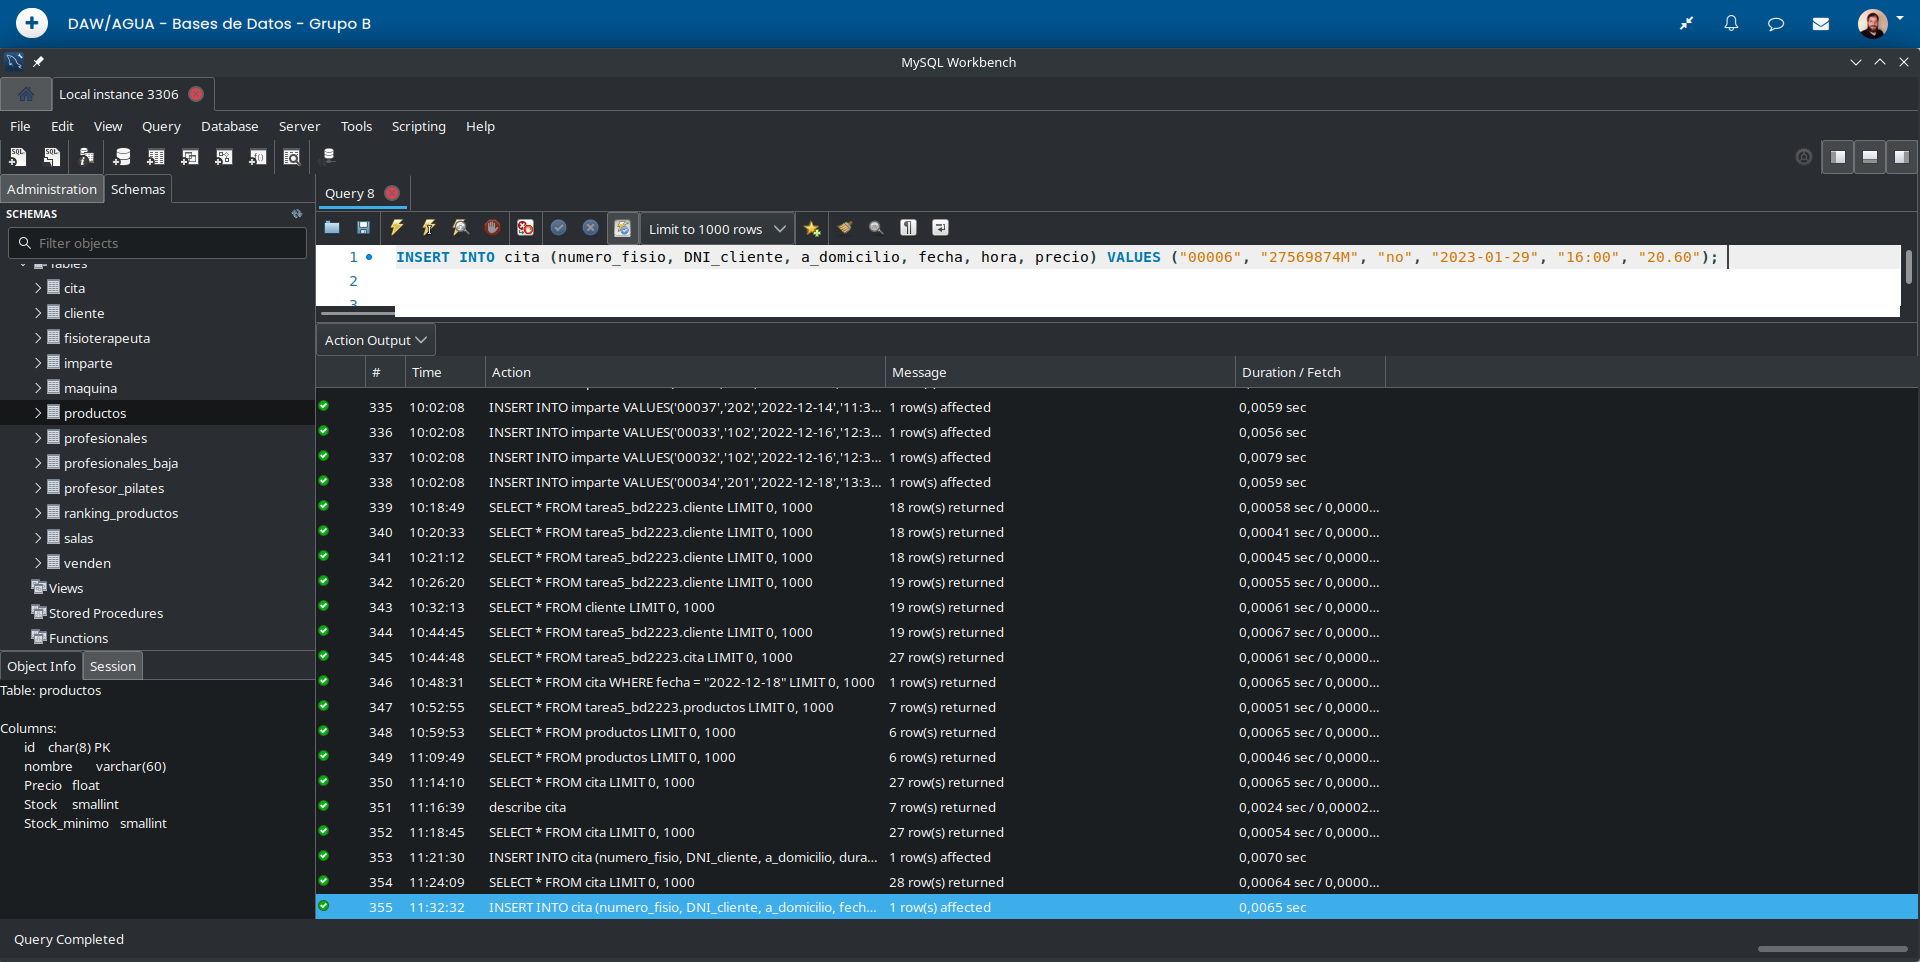
\includegraphics[scale=0.23]{sql-1.2.png}
            \caption{Ejecución de la segunda sentencia}
        \end{figure}

    \item \textbf{Tercera sentencia}:

    \begin{figure}[H]
        \begin{tcolorbox}[sharp corners, colback=yellow!30, colframe=white!20]
            \scriptsize
            \begin{verbatim}


INSERT INTO cita (numero_fisio, DNI_cliente, duracion, fecha, hora, precio)
VALUES ("00003", "73256987D", "01:00", "2023-02-02", "12:00", "40");
            \end{verbatim}
        \end{tcolorbox}
    \end{figure}

    \begin{figure}[H]
        \centering
        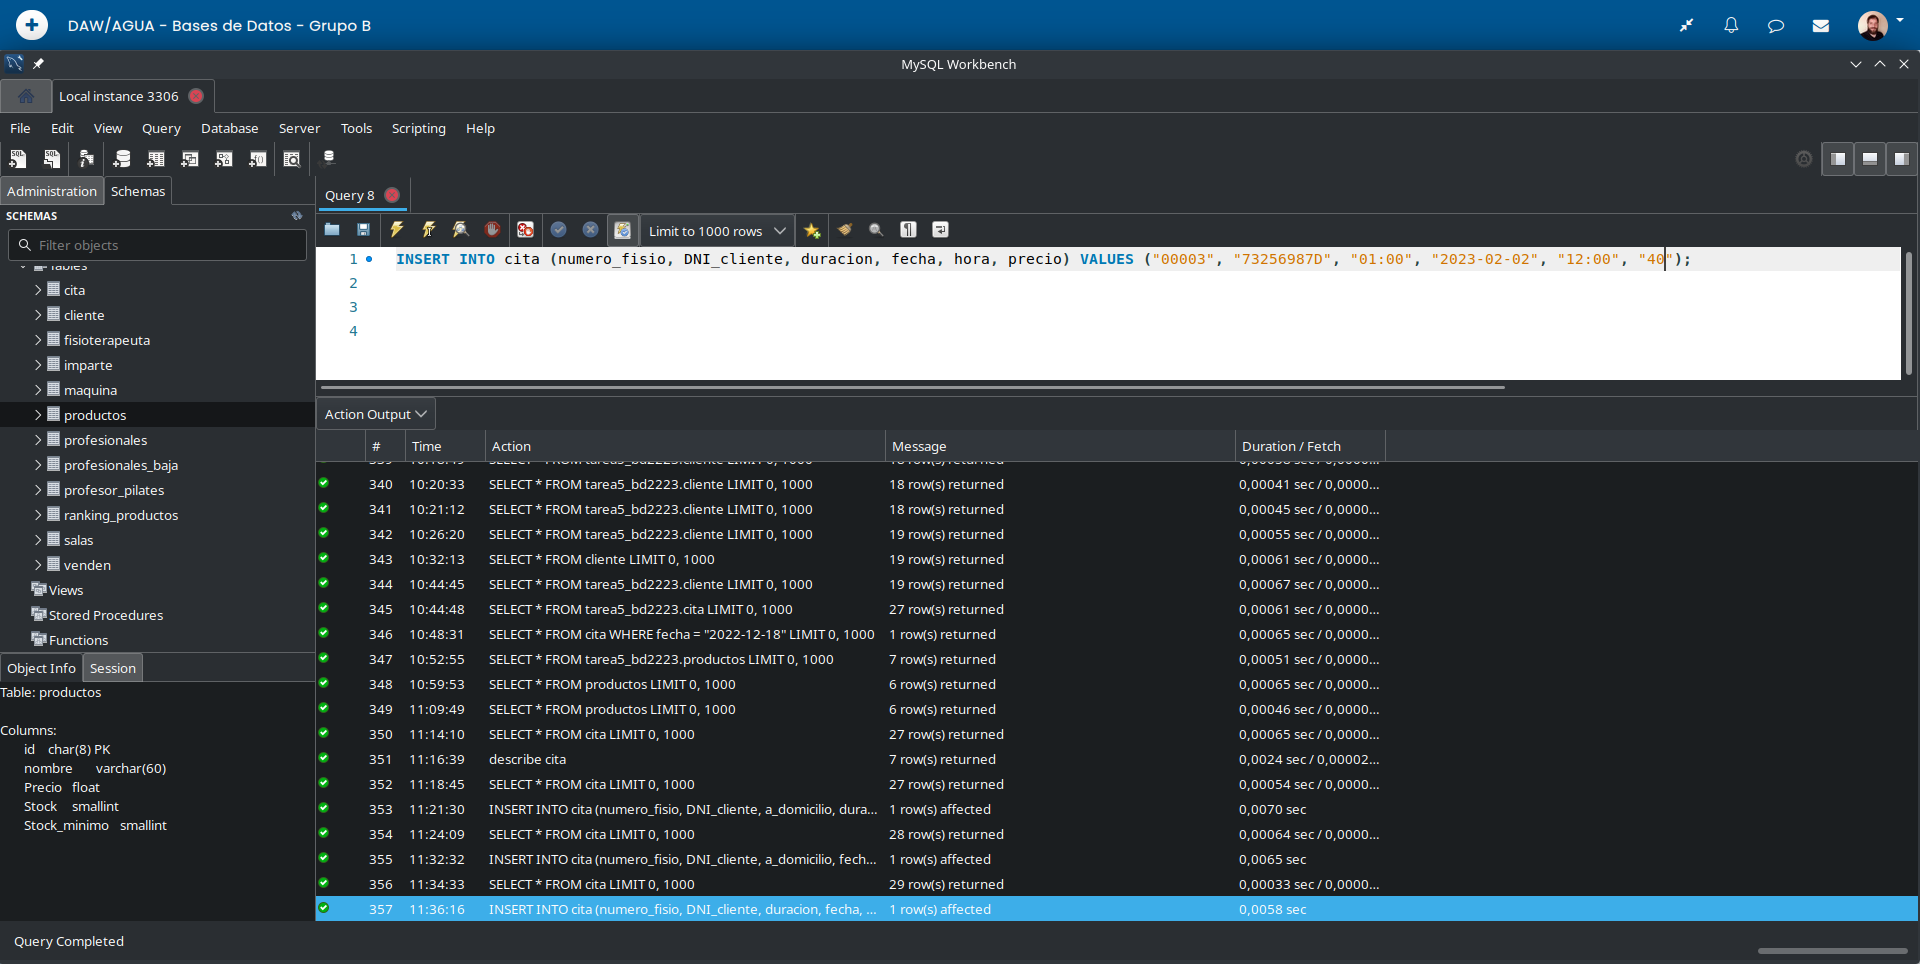
\includegraphics[scale=0.23]{sql-1.3.png}
        \caption{Ejecución de la tercera sentencia}
    \end{figure}
    \end{itemize}

    Una vez modificada la tabla \textbf{citas}, mostramos la tabla realizando una consulta \textbf{SELECT * FROM cita} para mostrar que todos los datos se han añadido correctamente.

    \begin{figure}[H]
        \centering
        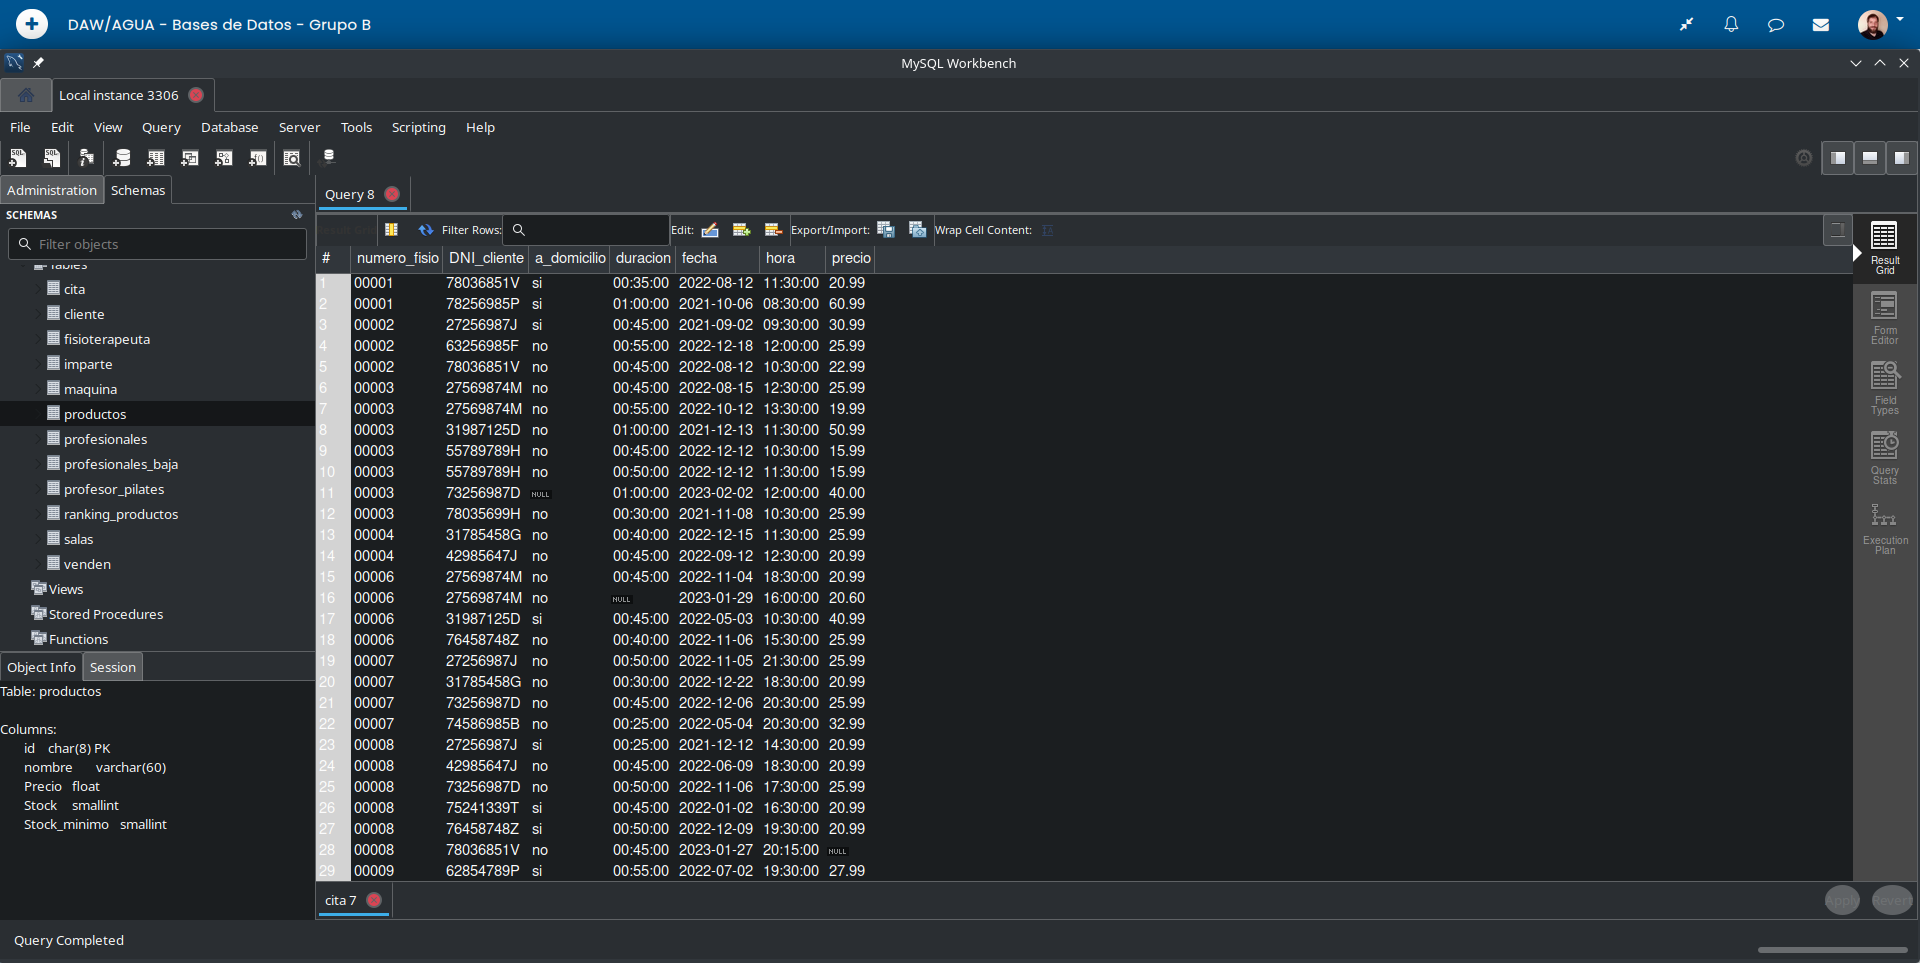
\includegraphics[scale=0.23]{sql-1.4.png}
        \caption{Tabla citas con los nuevos registros añadidos}
    \end{figure}


    \item En este punto vamos a incrementar el precio de los vendajes en la tabla productos un 15\%. Recordemos, que para trabajar con Workbench, debemos haber deshabilitado la opción \textbf{sql\_safe\_update}, desde el menú \textbf{Preferences -> SQL Editor}.

       \begin{figure}[H]
        \begin{tcolorbox}[sharp corners, colback=yellow!30, colframe=white!20]
            \scriptsize
            \begin{verbatim}


UPDATE productos SET precio = precio + ROUND((precio*15)/100, 2) WHERE nombre LIKE "%Vendaje%";
            \end{verbatim}
        \end{tcolorbox}
    \end{figure}

    En la siguiente imagen se puede ver como la sentencian se ha ejecutado correctamente, afectando a 3 filas.

    \begin{figure}[H]
        \centering
        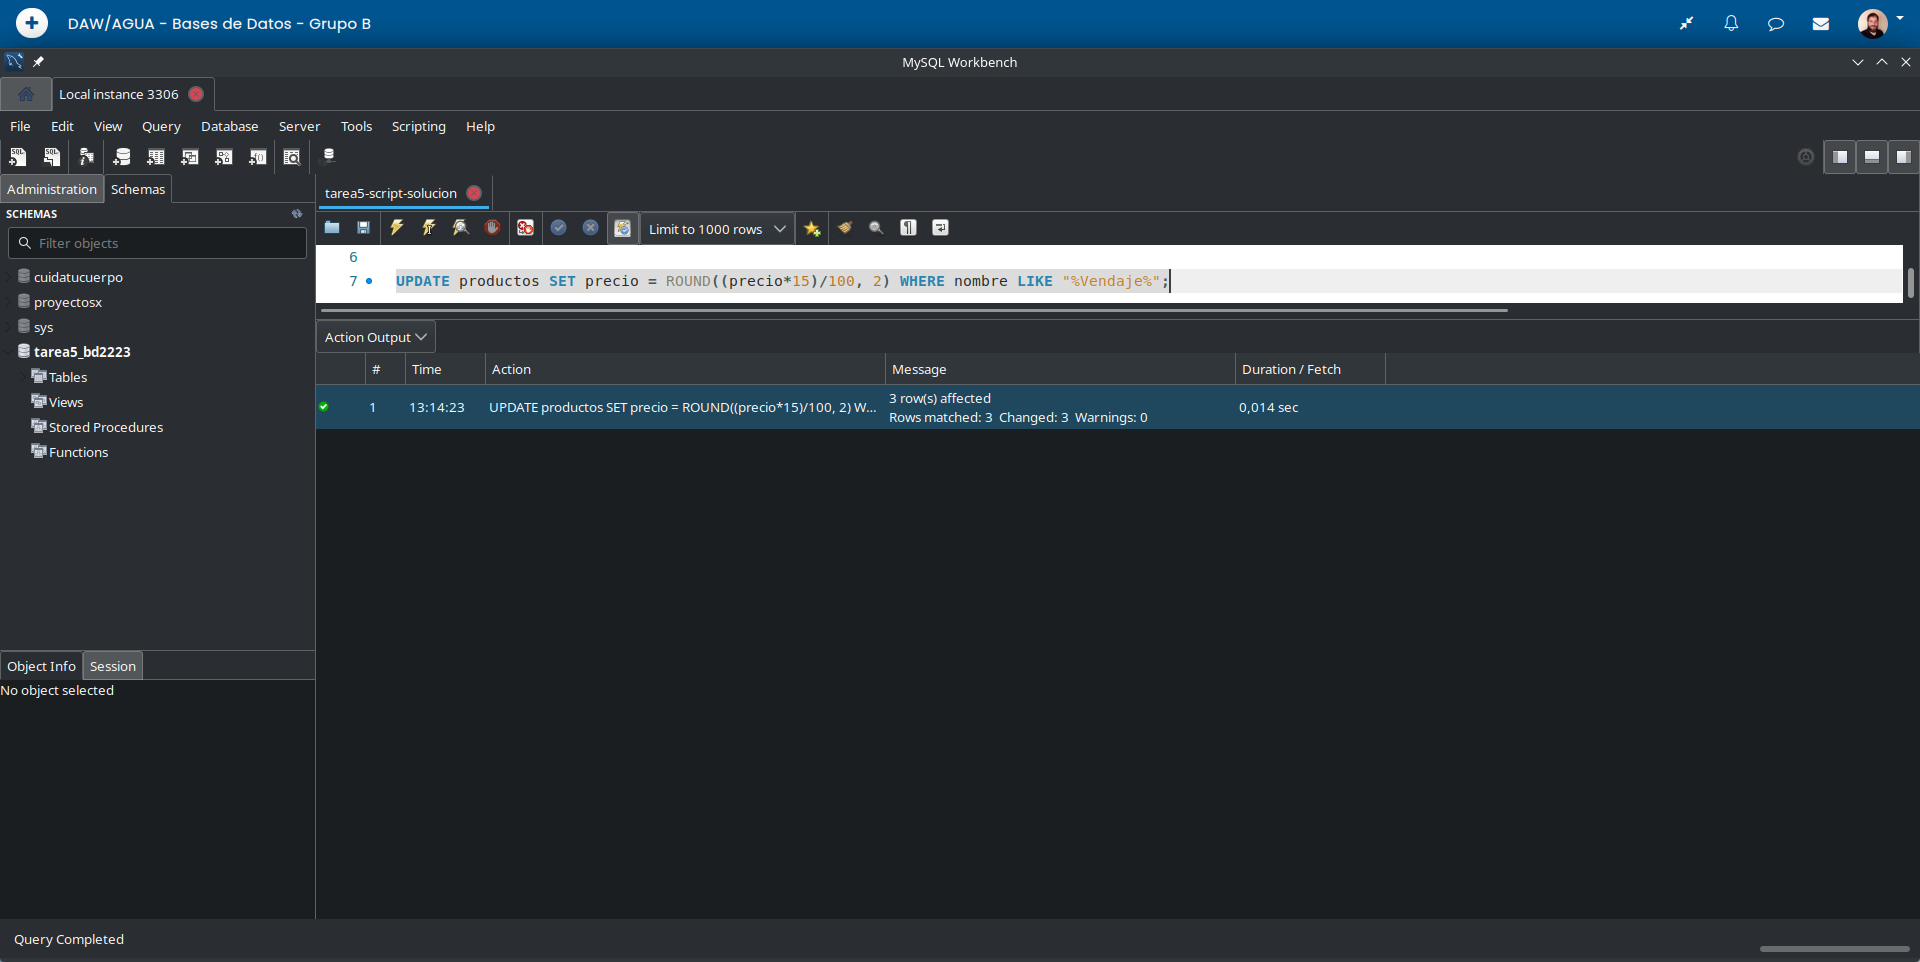
\includegraphics[scale=0.23]{sql-2.1.png}
        \caption{Ejecución de la sentencia de actualización}
    \end{figure}

    Para comprobar que se han actualizado, hemos consultado la tabla productos, donde podemos ver el precio de los vendajes actualizado.

     \begin{figure}[H]
        \centering
        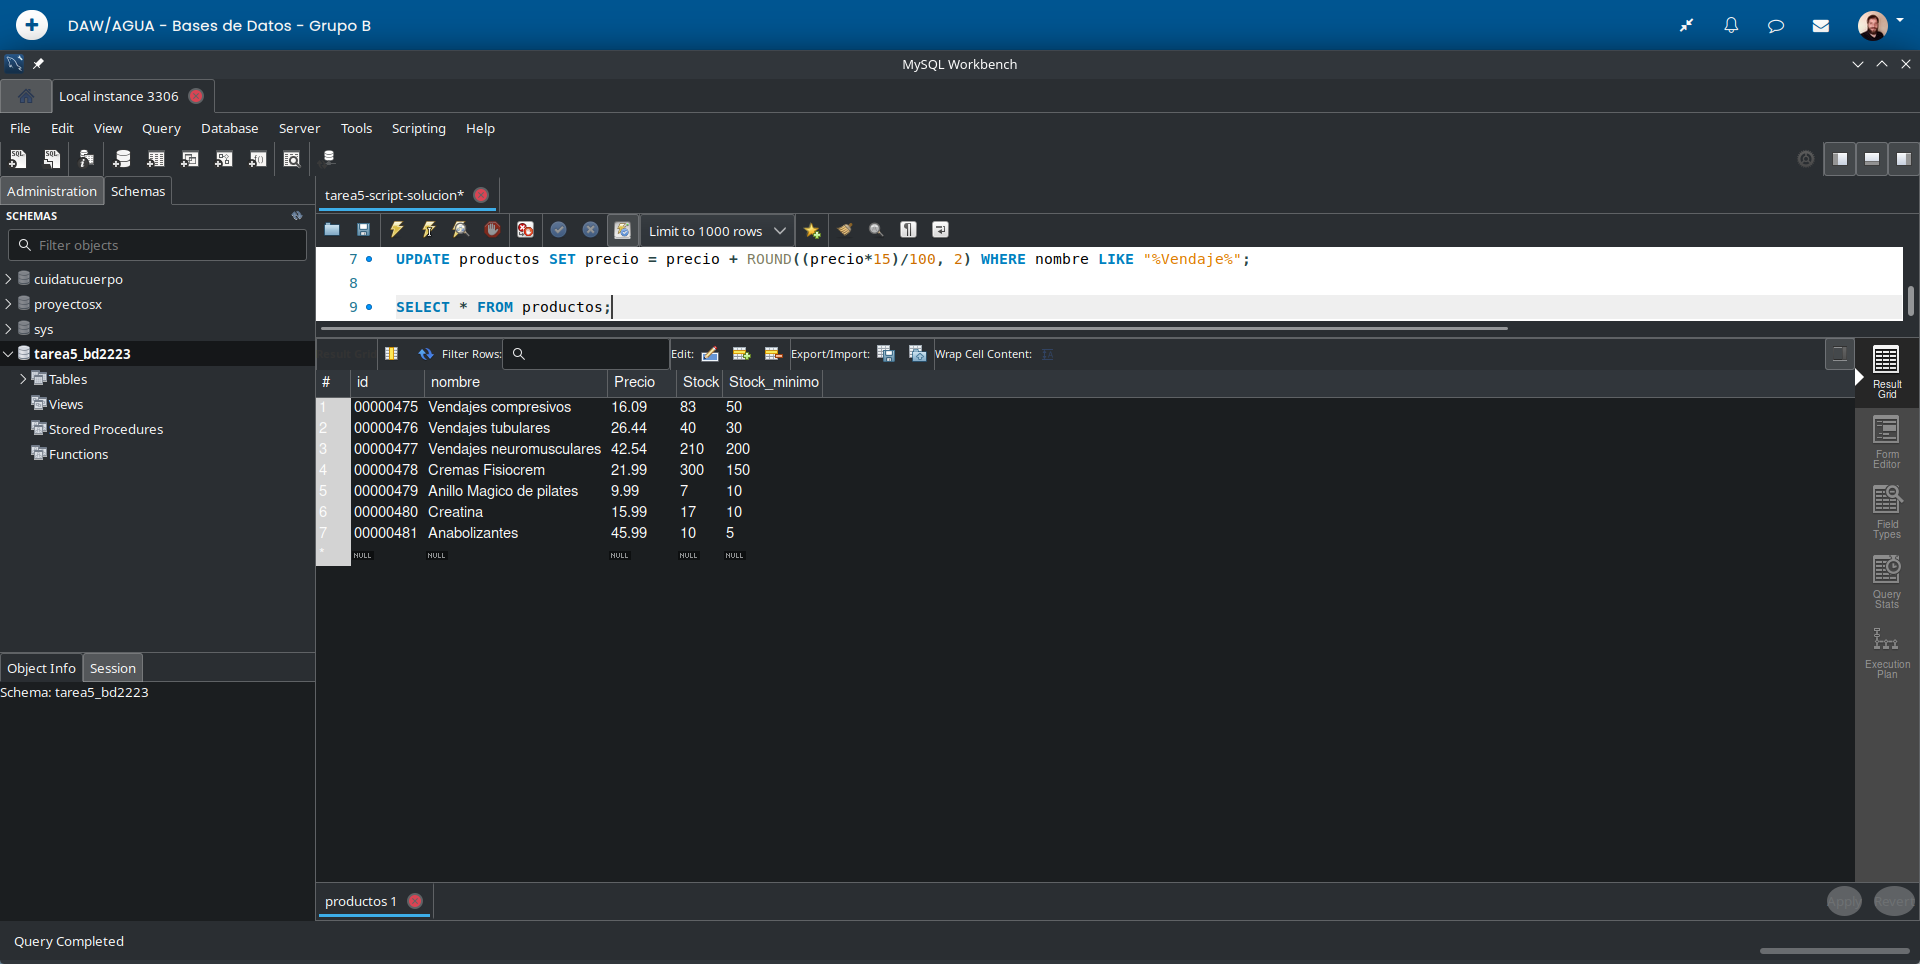
\includegraphics[scale=0.23]{sql-2.2.png}
        \caption{Precio de los vendajes actualizado en la tabla productos}
    \end{figure}

    \item Ahora vamos a modificar la tabla citas para eliminar aquellas que valgan menos de 25€ y que además estén asignadas a profesionales que no estén trabajando. La sentencia empleada es la siguiente.


    \begin{figure}[H]
        \begin{tcolorbox}[sharp corners, colback=yellow!30, colframe=white!20]
            \scriptsize
            \begin{verbatim}


DELETE FROM cita
WHERE numero_fisio
IN (SELECT  numero_trabajador FROM profesionales WHERE estado IN ("Ausente", "Despedido"))
AND precio < 25;
            \end{verbatim}
        \end{tcolorbox}
    \end{figure}

    La sentencia se ha ejecutado afectando a 2 filas, como podemos ver en la siguiente captura.

    \begin{figure}[H]
        \centering
        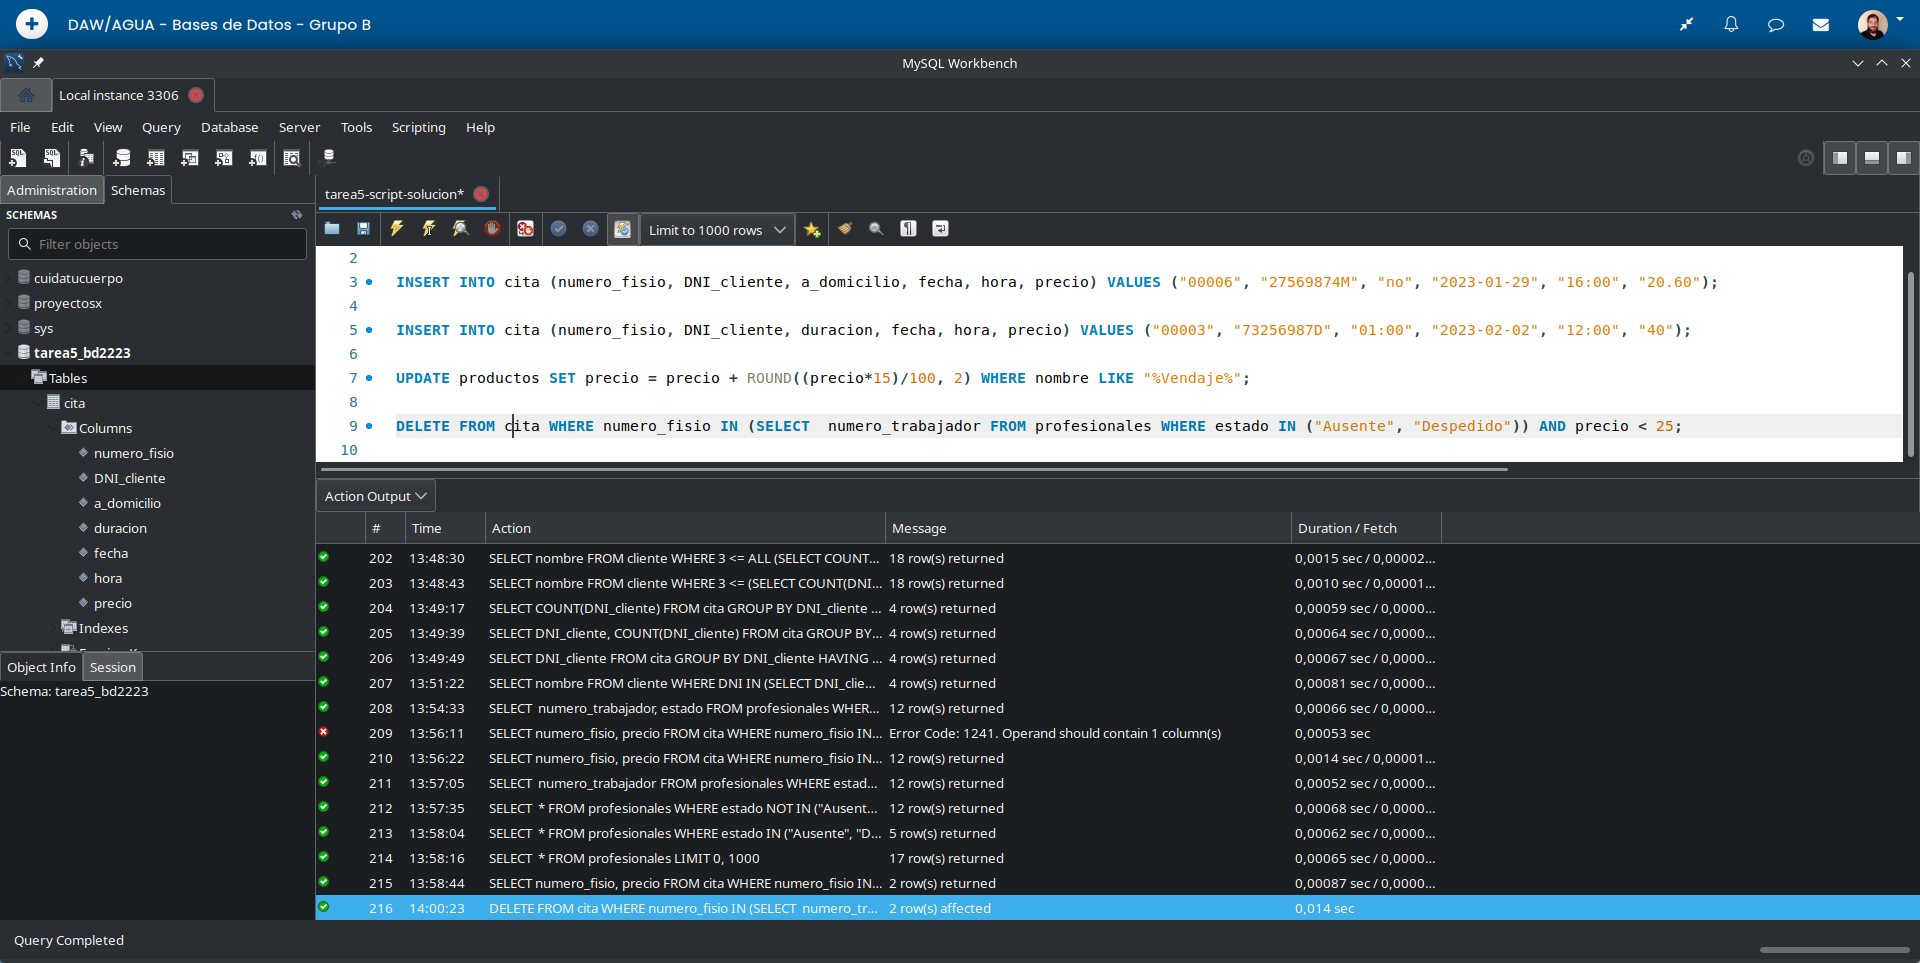
\includegraphics[scale=0.23]{sql-3.1.png}
        \caption{Ejecución de borrado de citas}
    \end{figure}

    Para comprobarlo, hemos seleccionado todas las citas mediante una consulta para comprobar que se han borrado correctamente.

    \begin{figure}[H]
        \centering
        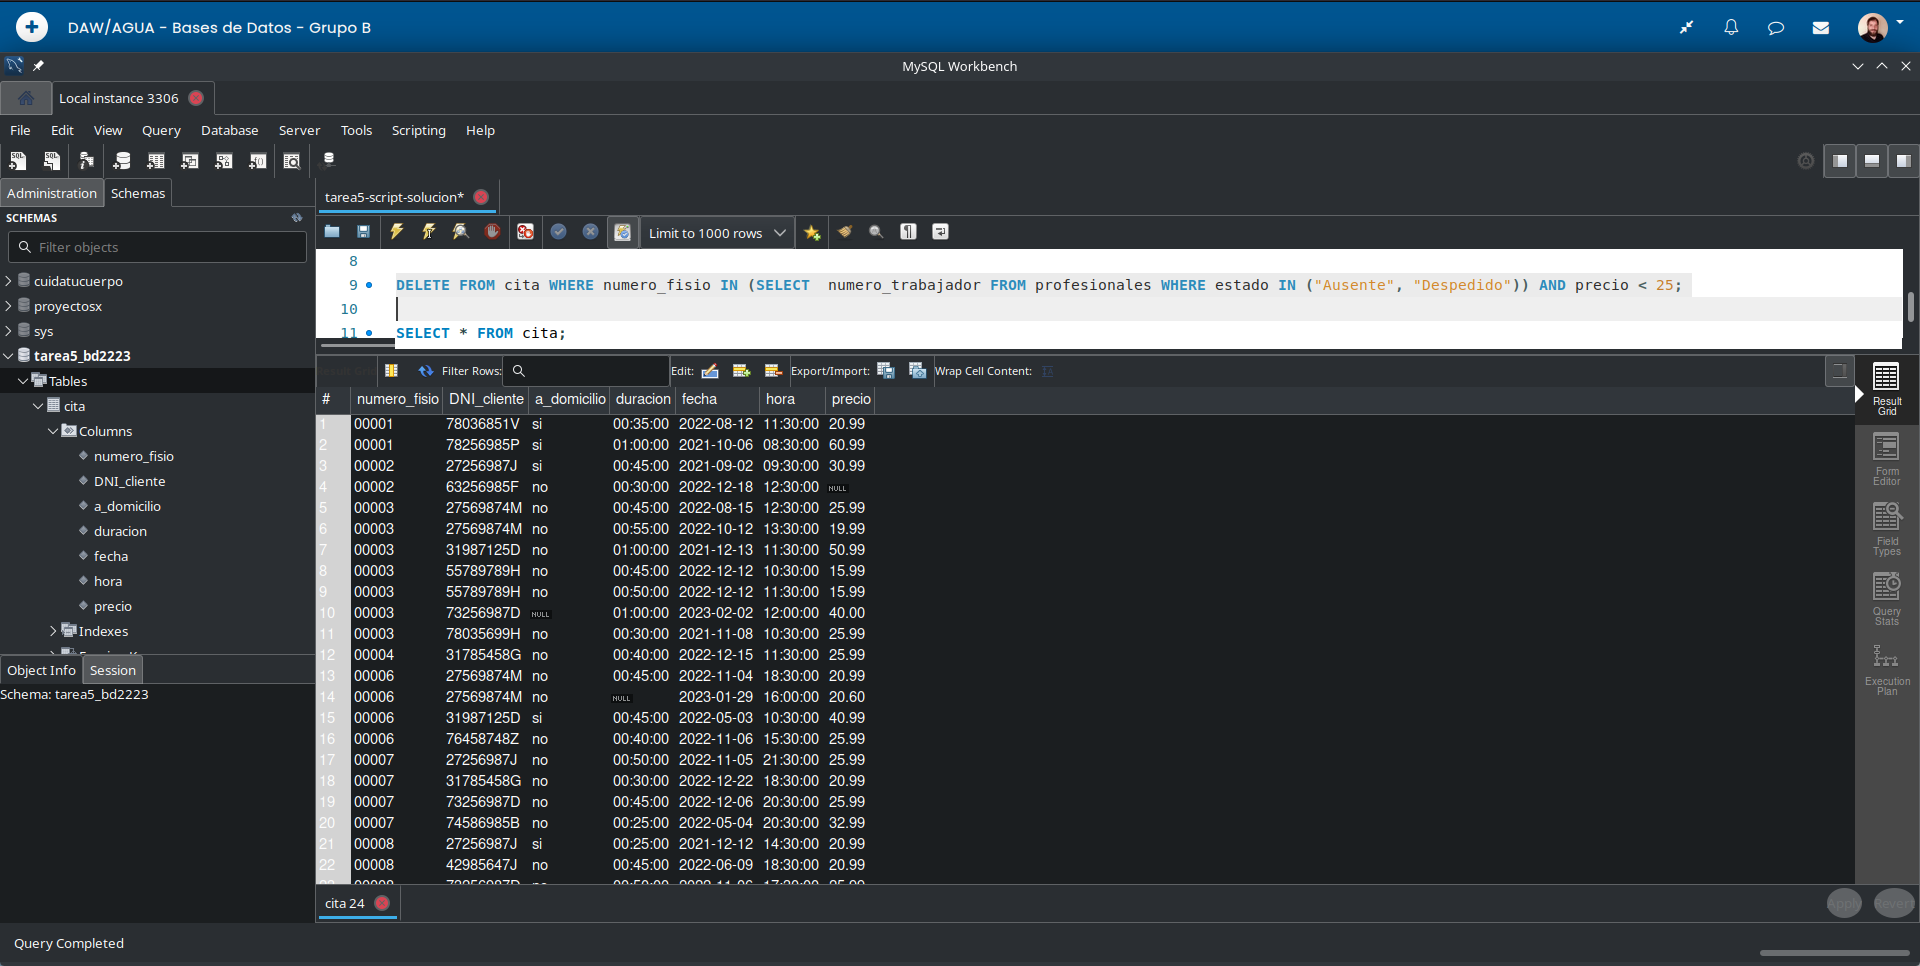
\includegraphics[scale=0.23]{sql-3.2.png}
        \caption{Citas borradas correctamente de la tabla}
    \end{figure}

    \item En este punto hemos actualizado el descuento de los clientes que hayan tenido 3 citas o más y tengan un descuento inferior al 60\%. La sentencia usada es la siguiente:

     \begin{figure}[H]
        \begin{tcolorbox}[sharp corners, colback=yellow!30, colframe=white!20]
            \scriptsize
            \begin{verbatim}

            UPDATE cliente SET descuento = descuento + 5
            WHERE DNI IN
                (SELECT DNI_cliente FROM cita
                 WHERE YEAR(fecha) = 2022
                 GROUP BY DNI_cliente
                 HAVING COUNT(DNI_cliente) > 2)
            AND descuento < 60;
            \end{verbatim}
        \end{tcolorbox}
    \end{figure}

    La sentencia se ha ejecutado correctamente y se han actualizado 1 filas, como vemos en la siguiente figura.

    \begin{figure}[H]
        \centering
        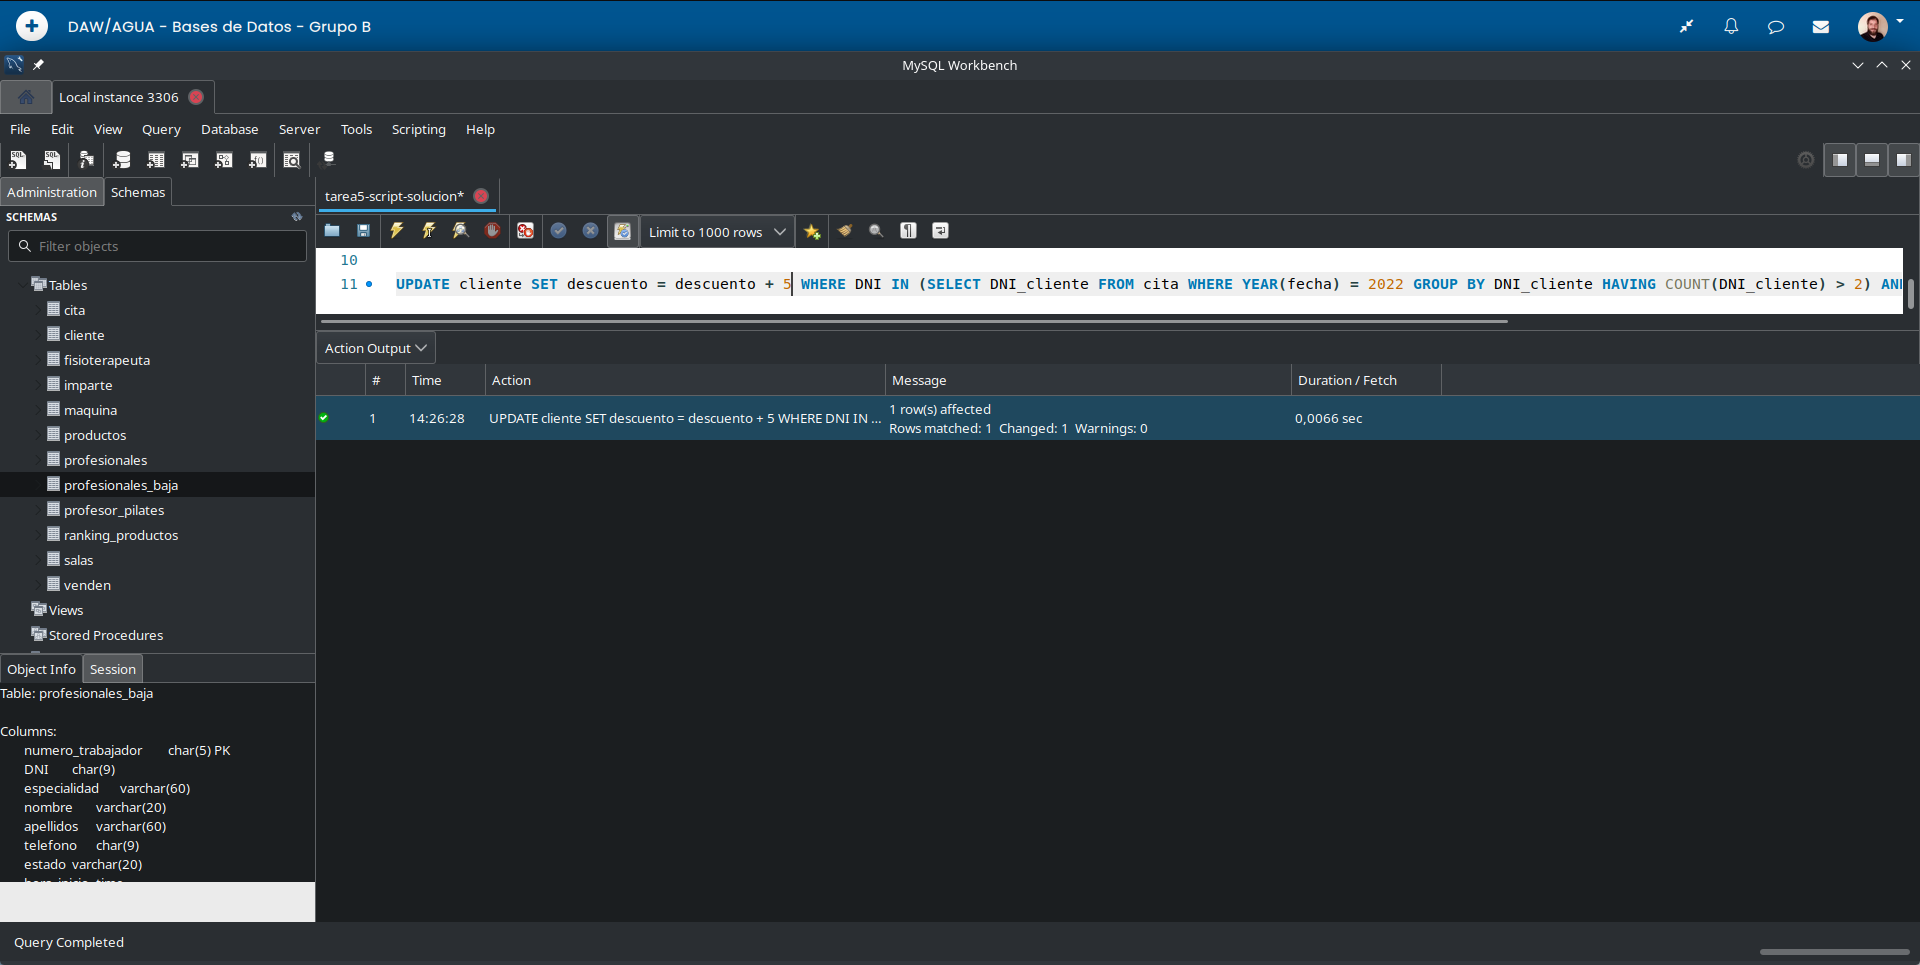
\includegraphics[scale=0.23]{sql-4.1.png}
        \caption{Actualización del descuento en la tabla cliente}
    \end{figure}

    Una vez ejecutada, hemos hecho una consulta, sobre el cliente que debería tener actualizado el descuento, para comprobar que se ha modificado correctamente.

    \begin{figure}[H]
        \centering
        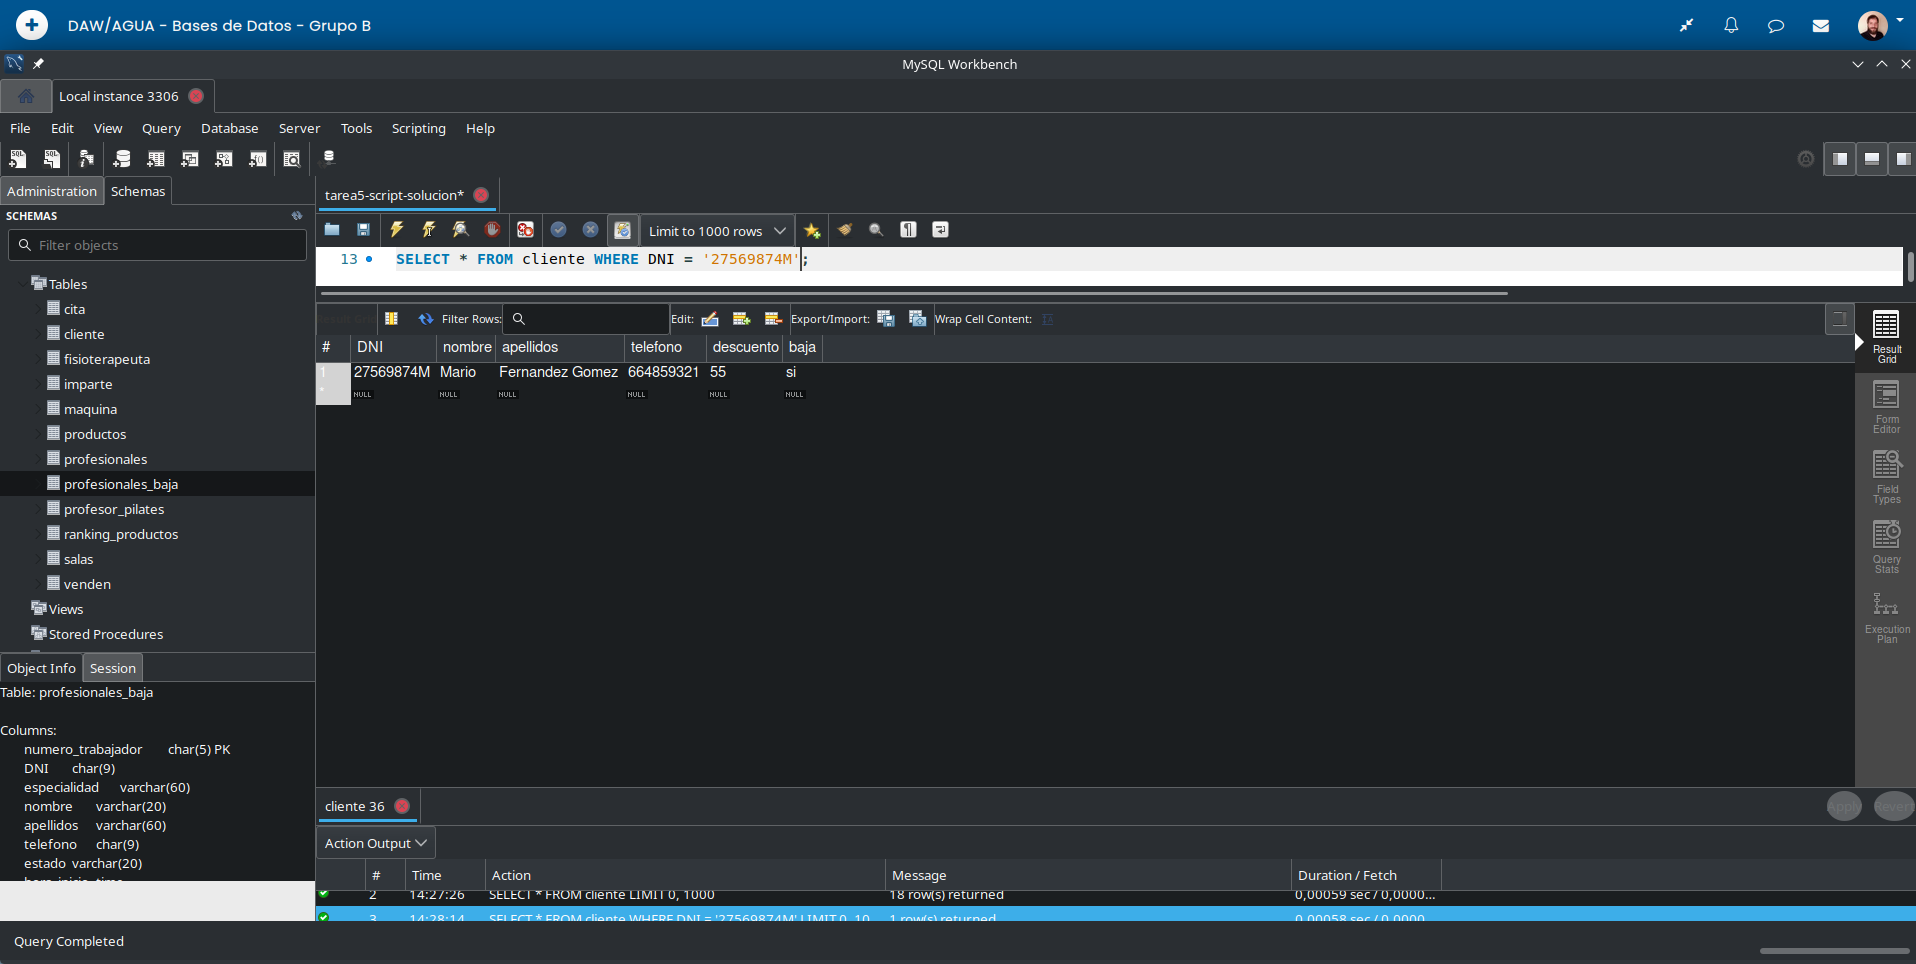
\includegraphics[scale=0.23]{sql-4.2.png}
        \caption{Cliente con el descuento actualizado correctamente}
    \end{figure}

    \item Vamos a incluir todos los profesionales que estén despedidos dentro de la tabla profesionales\_baja. Para ello, hemos usado la siguiente sentencia:

    \begin{figure}[H]
        \begin{tcolorbox}[sharp corners, colback=yellow!30, colframe=white!20]
            \scriptsize
            \begin{verbatim}

            INSERT INTO profesionales_baja
            SELECT
                numero_trabajador,
                DNI,
                especialidad,
                nombre,
                apellidos,
                telefono,
                estado,
                hora_inicio,
                hora_fin,
                hora_fin - hora_inicio
            FROM profesionales
            WHERE estado = "Despedido";
            \end{verbatim}
        \end{tcolorbox}
    \end{figure}

    Esta sentencia ha añadido 4 registros a la tabla profesionales baja, como podemos ver en la siguiente captura.

    \begin{figure}[H]
        \centering
        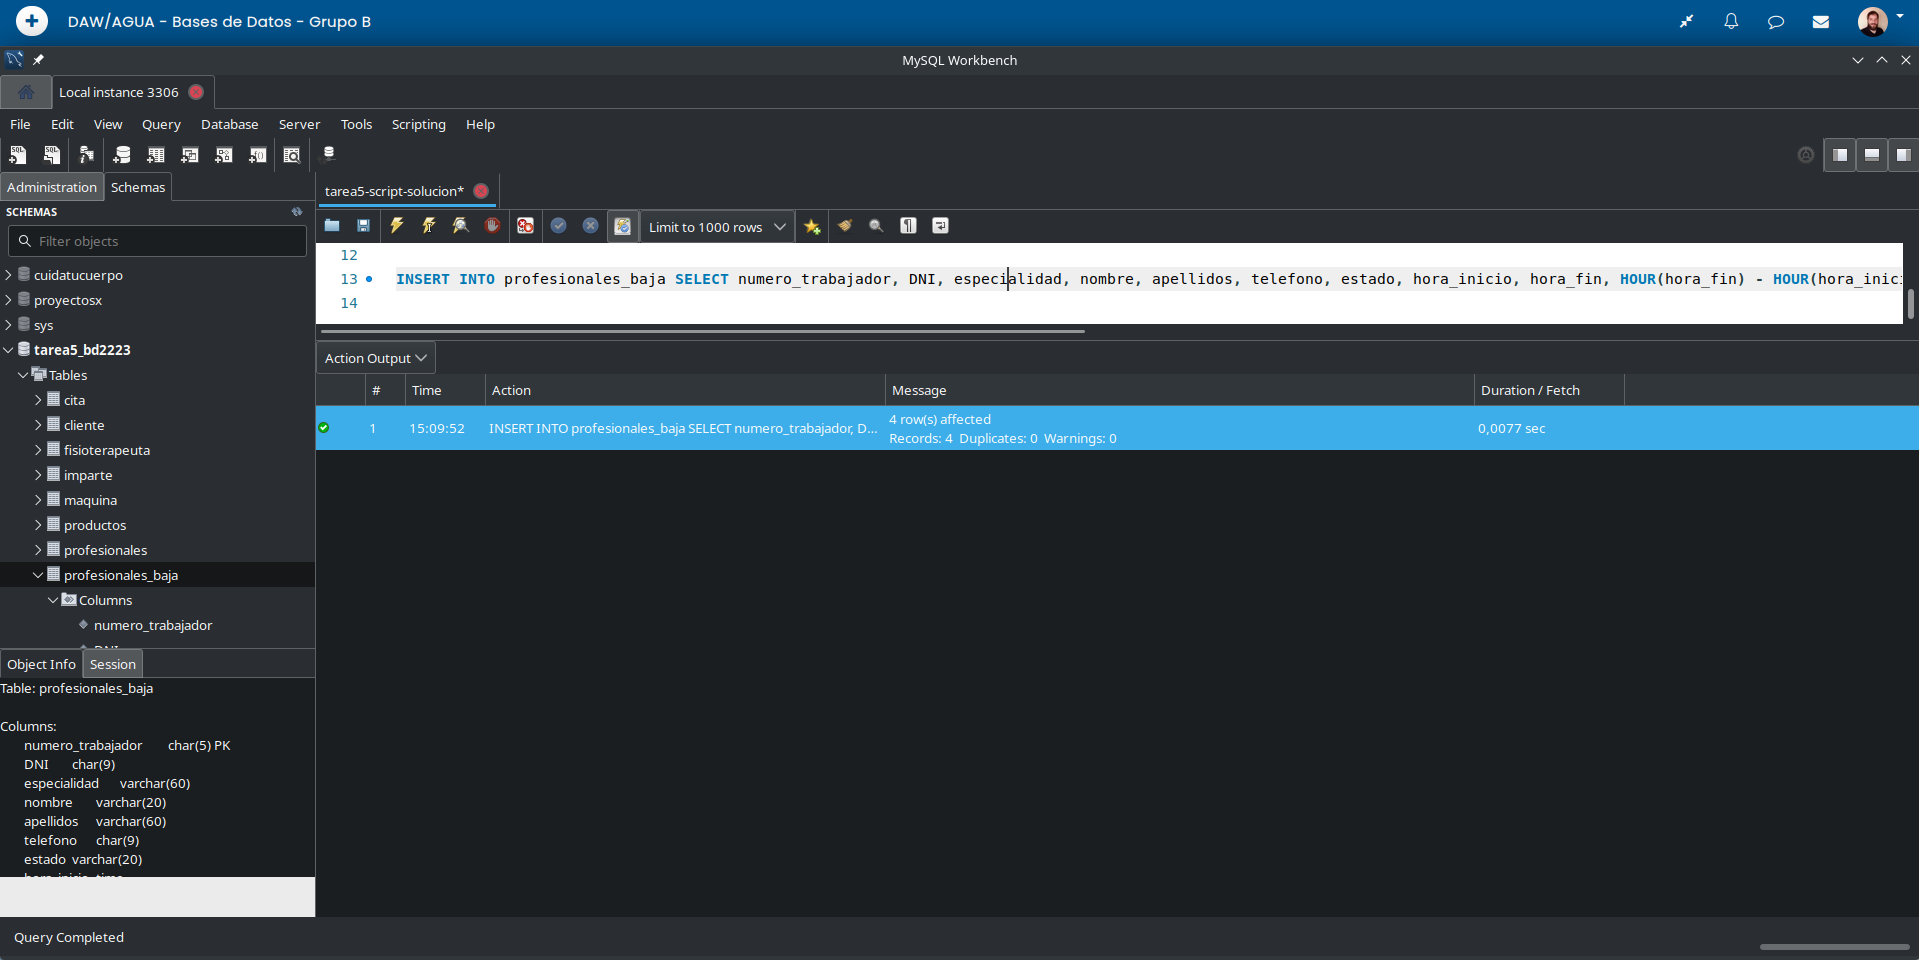
\includegraphics[scale=0.23]{sql-5.1.png}
        \caption{Adición de los profesionales despedidos a la tabla profesionales\_baja}
    \end{figure}

    A continuación, hemos consultado la tabla profesionales\_baja para comprobar que se han creado los registros correctamente.

    \begin{figure}[H]
        \centering
        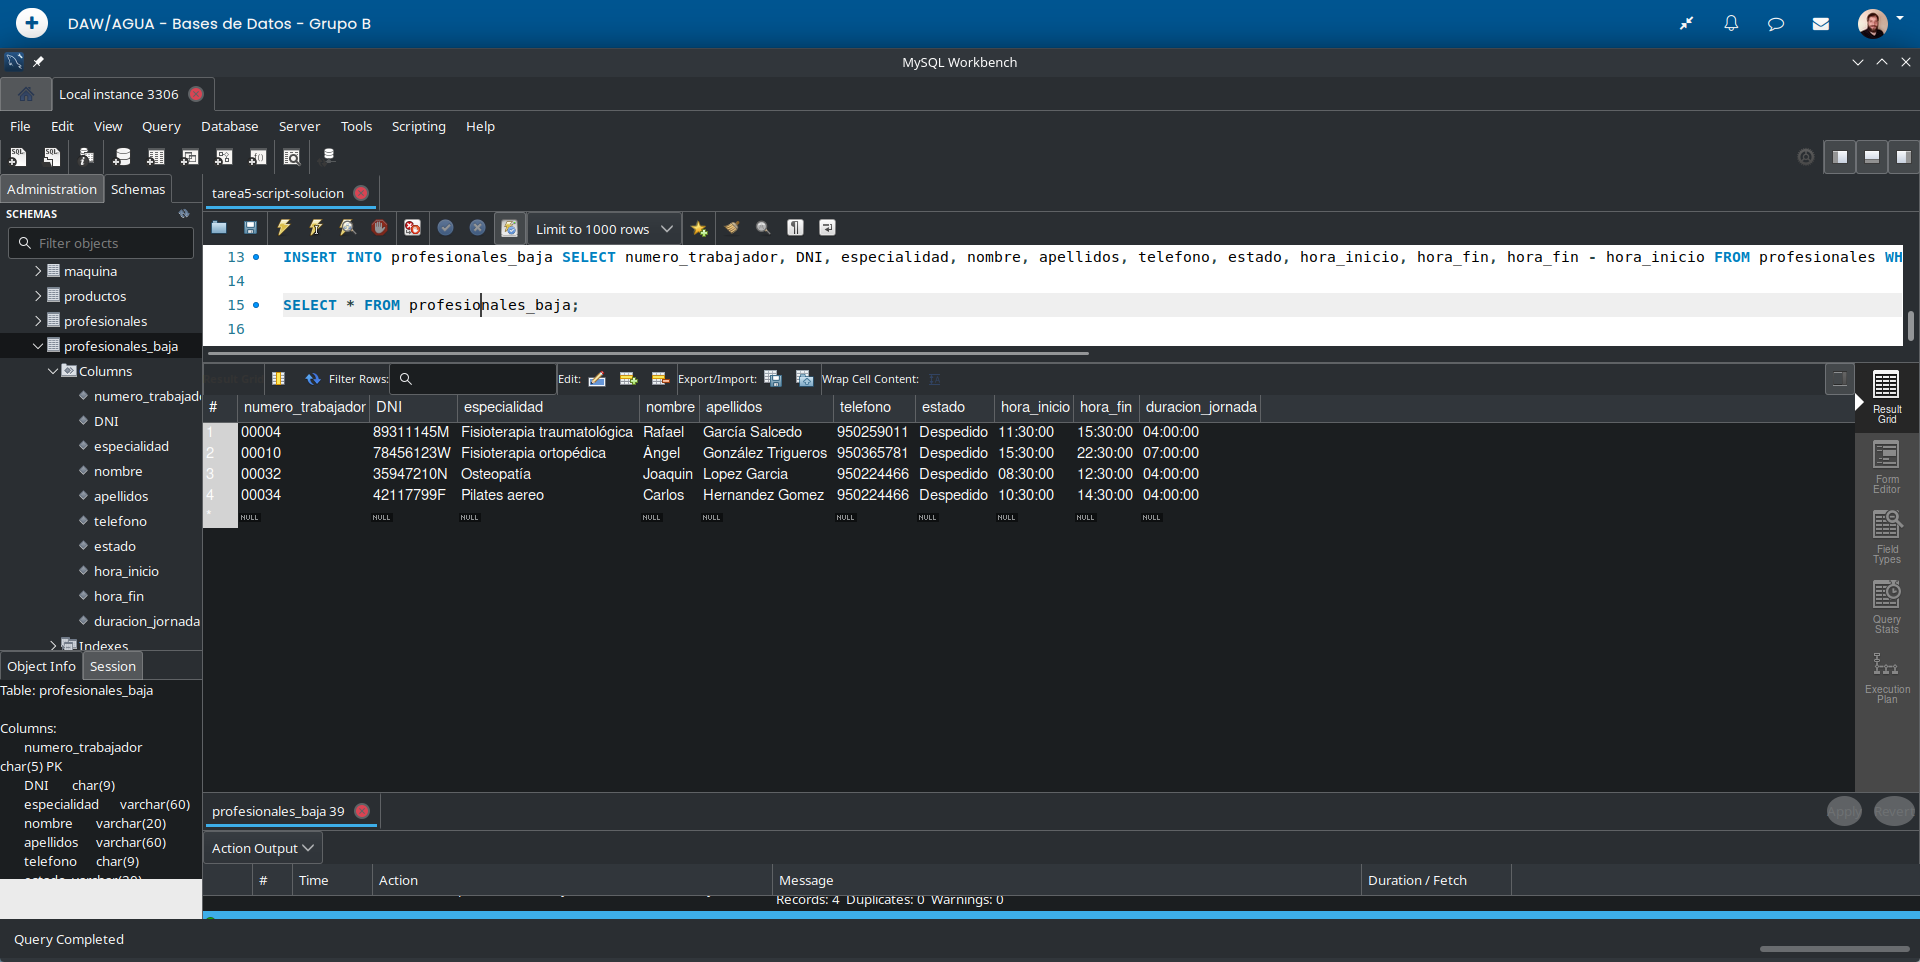
\includegraphics[scale=0.23]{sql-5.2.png}
        \caption{Registros creados en la tabla profesionales\_baja}
    \end{figure}

    \item En este punto vamos a decrementar la experiencia de los profesionales de pilates que haya impartido menos de 3 clases en el último año. Para ello, hemos empleado la siguiente sentencia:
\end{enumerate}

% Bibliography

%\newpage
%\bibliography{citas}
%\bibliographystyle{unsrt}

\end{document}